
\chapter{Appendix}
\section{Physiological Recording and Feature Extraction}
\label{app:physio}

\subsection{Sensor Placement}
Physiological signals were recorded using the Biofeedback~2000~Xpert system (Schuhfried GmbH).
The BVP sensor was attached to the index finger of the (left/right) hand, depending upon the user's non-dominant hand.
Electrodermal activity (EDA) electrodes were placed on the index fingers of the (left/right) hand.
Skin temperature was measured at the finger using the corresponding temperature sensor.
Participants were instructed to minimize hand and arm movements during recording.

\subsection{Acquisition and Synchronization}
All channels were recorded continuously throughout baseline, stress induction, meditation, and recovery phases.
Data were exported from the Biofeedback software in [format, e.g., .xls] and time-aligned with the experiment phases.

\subsection{Preprocessing and Artifact Handling}
Segments with obvious motion artifacts or signal dropouts were excluded from analysis.
If short missing sections occurred, they were handled by [removal / interpolation / not applicable].
No additional filtering was applied beyond the device/software default settings. % (edit if you did filtering)

\subsection{Feature Extraction}
Heart rate (HR) and inter-beat interval (IBI) were derived from the BVP signal.
Heart rate variability (HRV) was quantified using RMSSD, computed over [window length] for each phase.
EDA was summarized using the tonic skin conductance level (SCL) computed as the mean value per phase.
Phasic responses were quantified as SCR peaks detected using a threshold of [X] and a minimum inter-peak interval of [Y] seconds. % only if you actually did this
Skin temperature (TEMP) and pulse volume amplitude (PVA) were summarized using phase-wise mean values and changes relative to baseline.



\label{app:supp-figs}

\paragraph{Background music}
\label{sec:Music}
The background meditation music used in both experimental conditions was sourced from Pixabay
(\emph{``Relaxing Meditation (Tibetan Path)''}) \cite{pixabay_meditation_music}, which is distributed under the Pixabay Content License
and permits free use for academic and research purposes.


This appendix provides additional descriptive plots for all physiological signals,
including per-participant distributions and group-mean time courses.

\section{Heart Rate (HR)}

\begin{figure}[H]
    \centering
    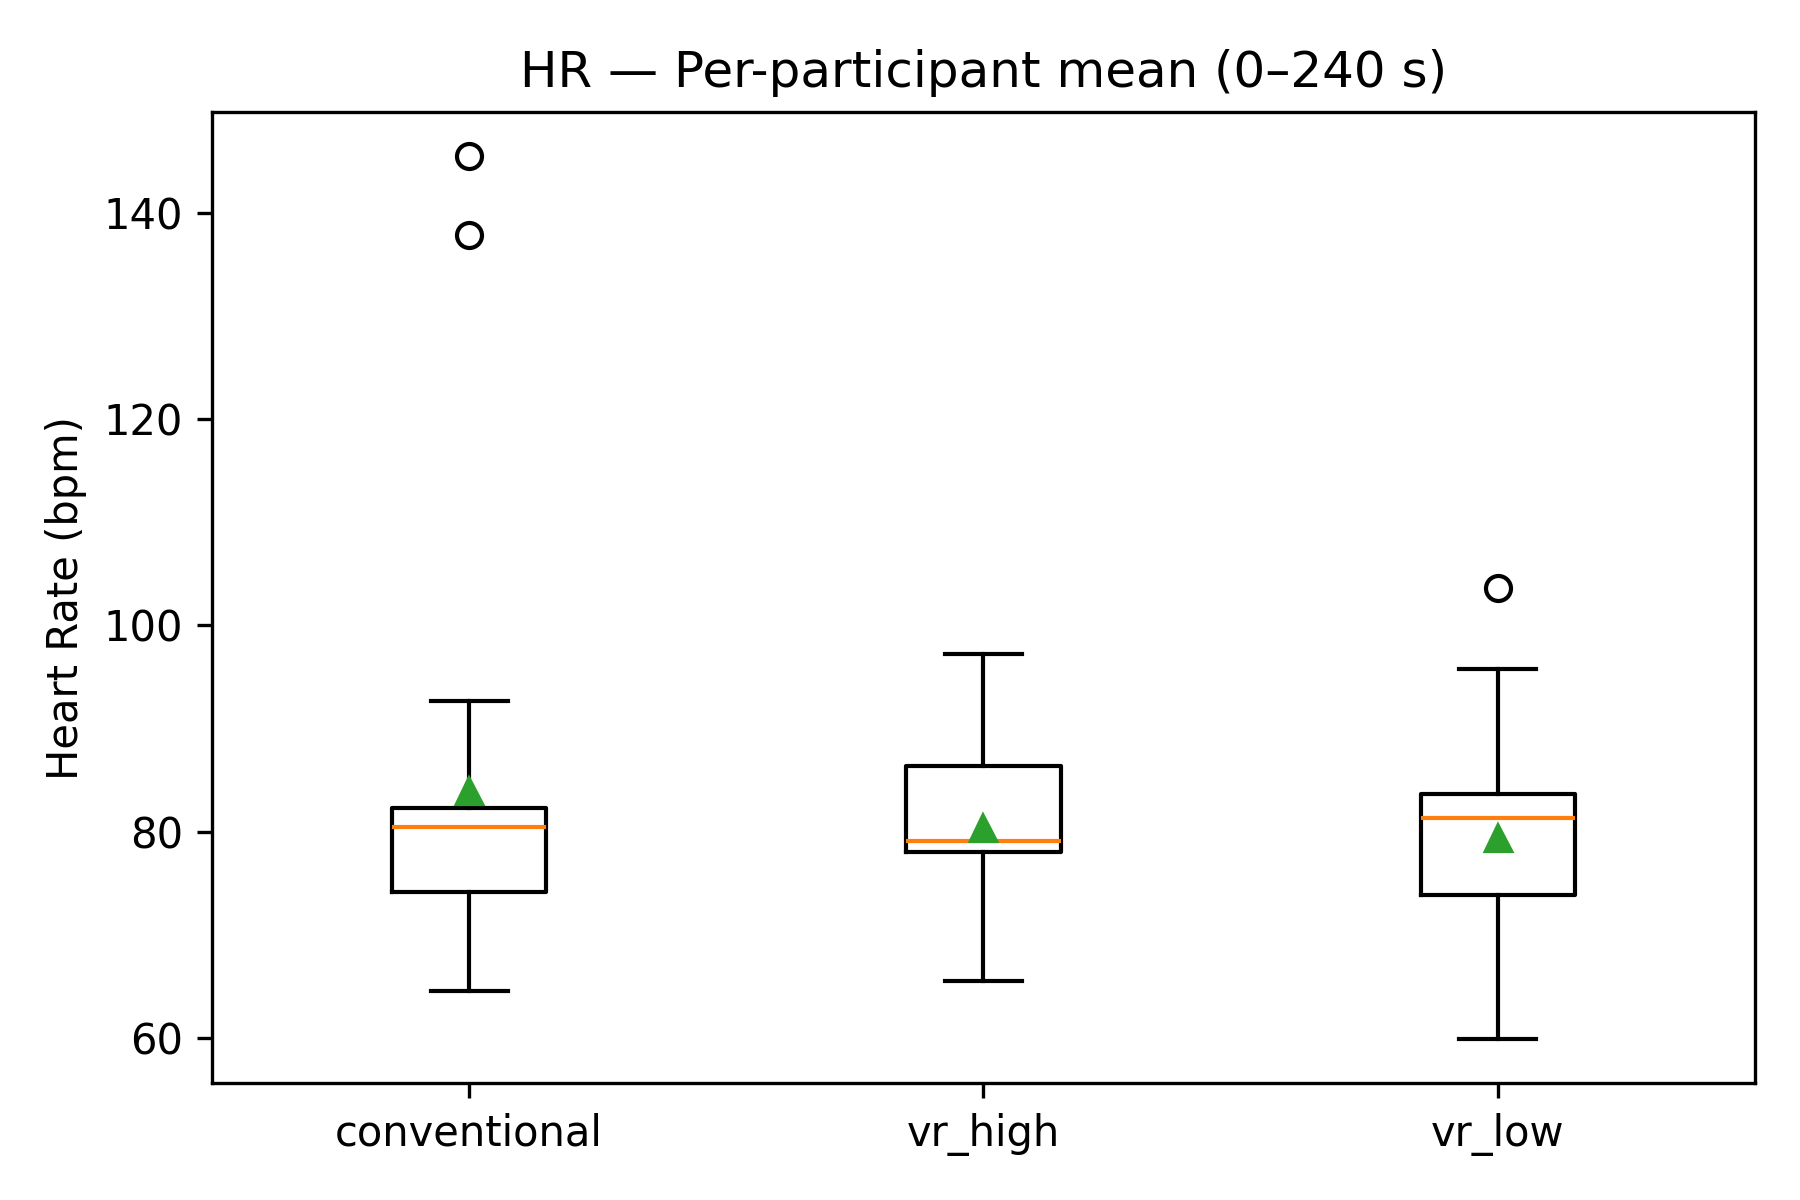
\includegraphics[width=\textwidth]{pics/result plots/boxplot_hr.png}
    \caption{Per-participant mean HR during meditation (all three groups).}
    \label{fig:hr-perparticipant-supp}
\end{figure}

\begin{figure}[H]
    \centering
    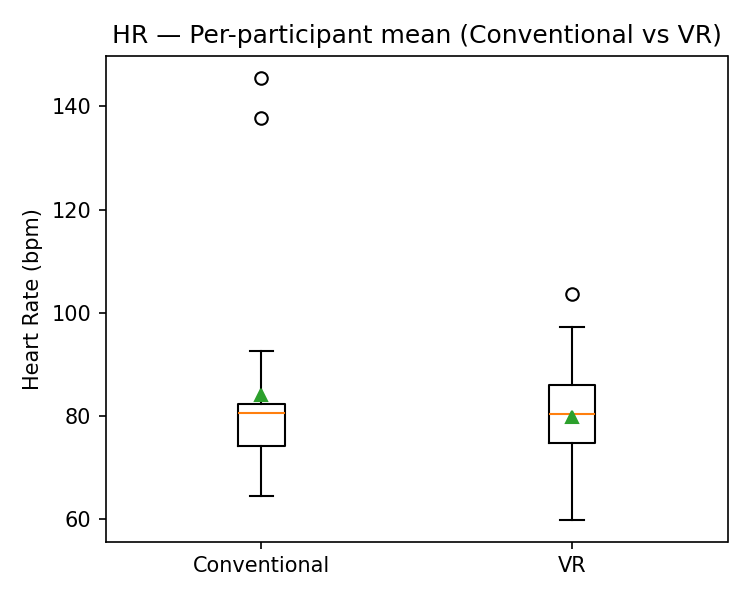
\includegraphics[width=\textwidth]{pics/result plots/box_collapsed_HR.png}
    \caption{Per-participant mean HR during meditation (Conventional vs.\ VR).}
    \label{fig:hr-perparticipant-convr}
\end{figure}

\begin{figure}[H]
    \centering
    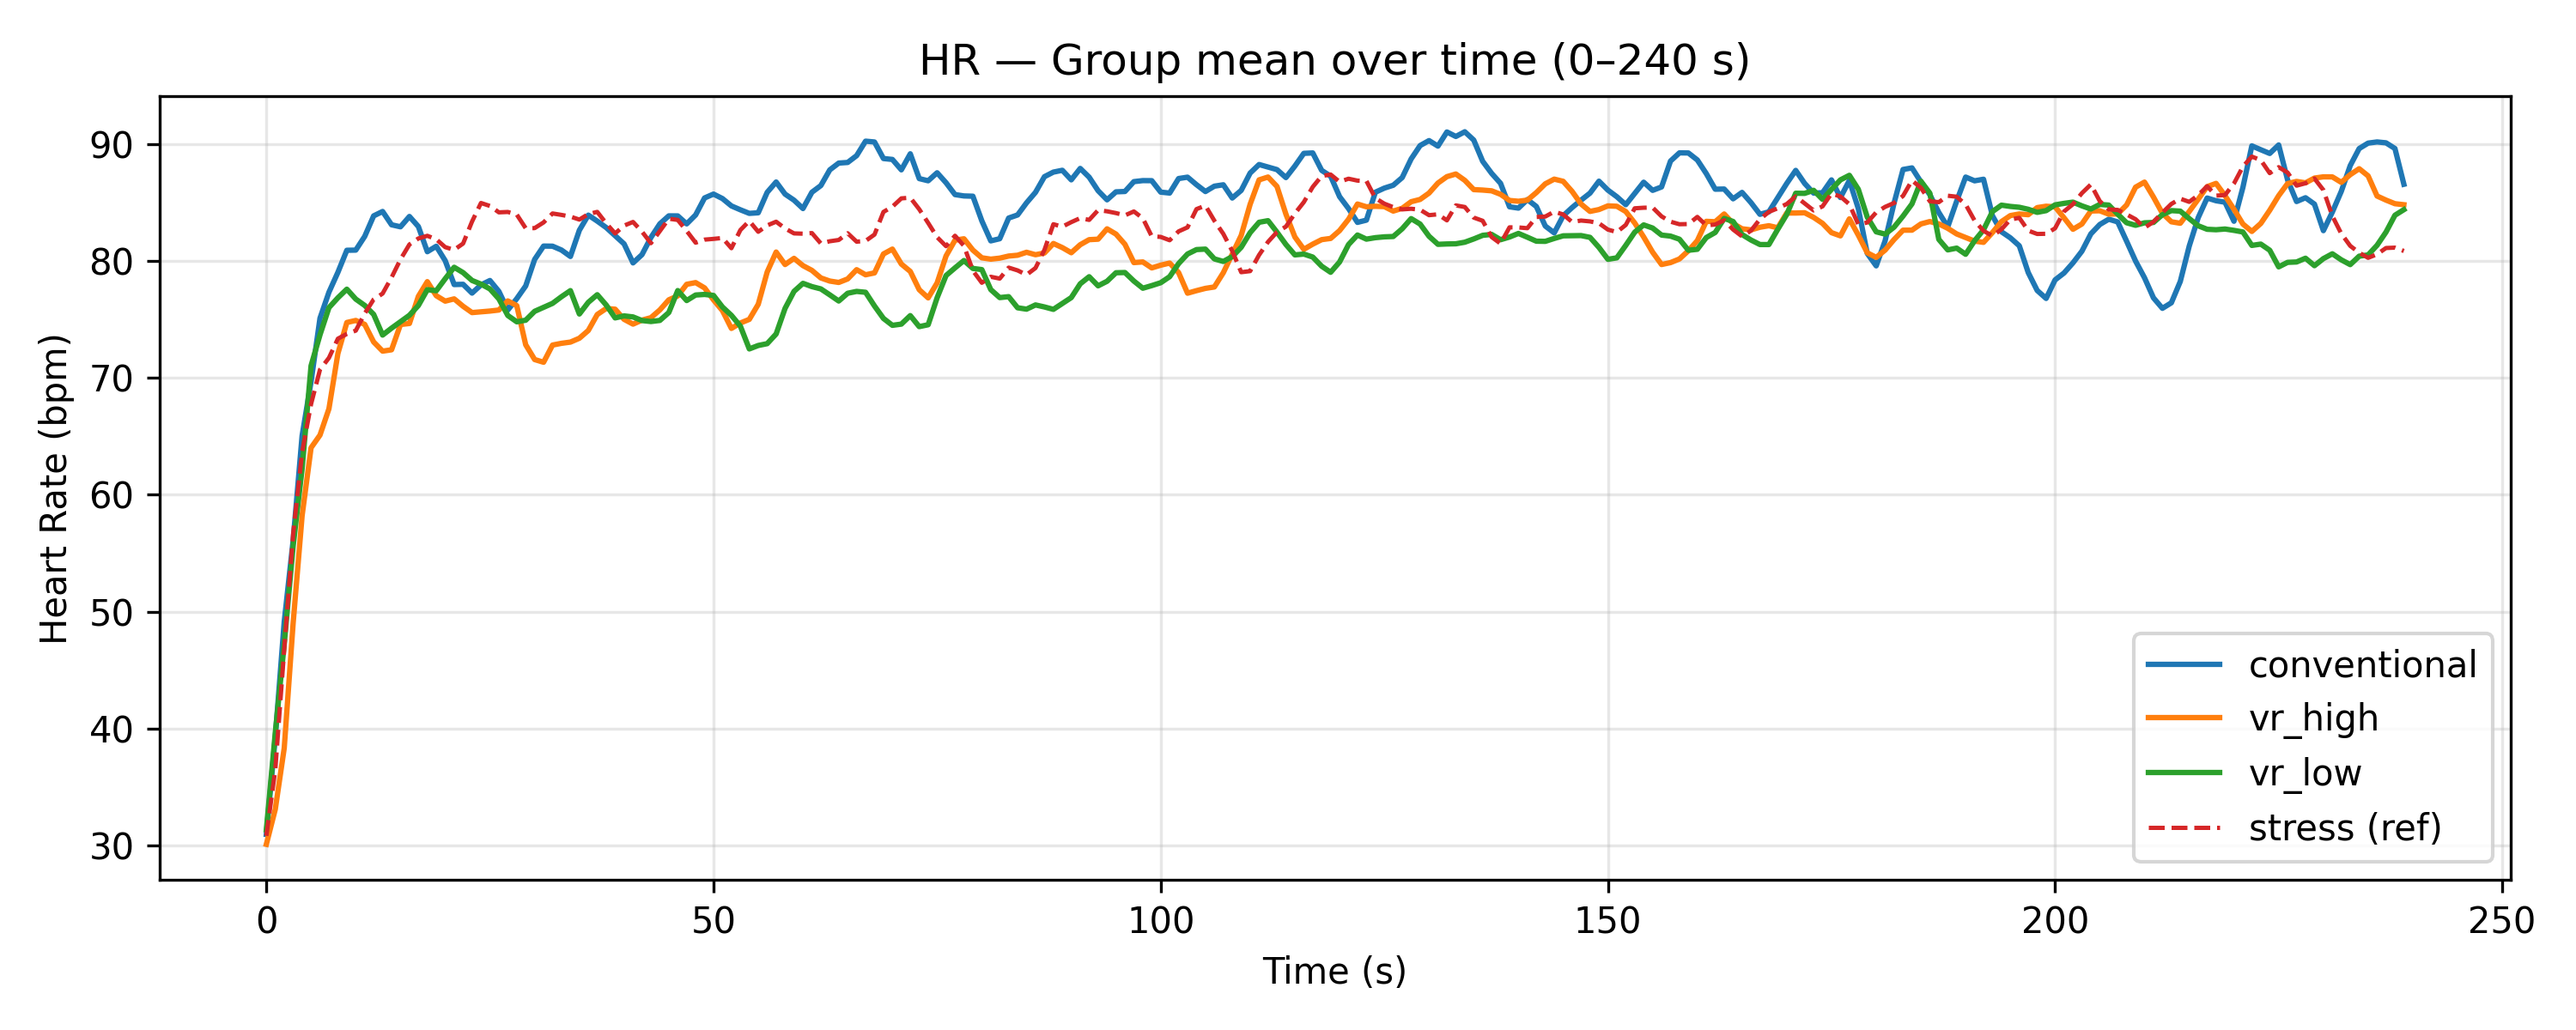
\includegraphics[width=\textwidth]{pics/result plots/timeseries_hr.png}
    \caption{Group-mean HR over time (0--240\,s) for all three groups.}
    \label{fig:hr-time-supp}
\end{figure}

\begin{figure}[H]
    \centering
    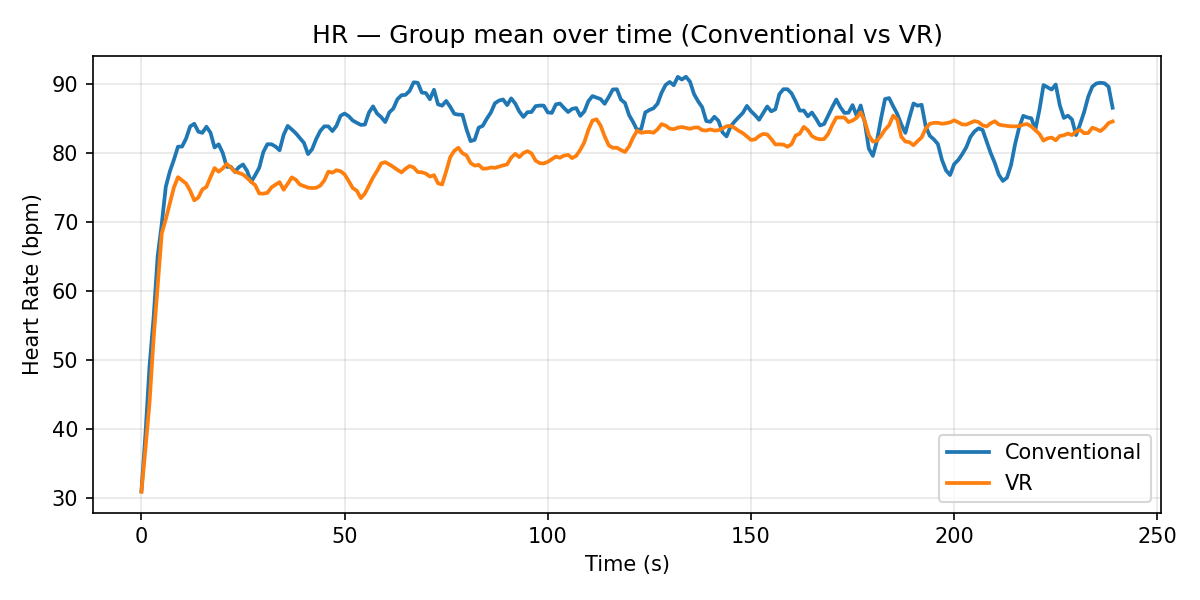
\includegraphics[width=\textwidth]{pics/result plots/lines_collapsed_HR.png}
    \caption{Group-mean HR over time (0--240\,s) for Conventional vs.\ VR.}
    \label{fig:hr-time-convr}
\end{figure}

\section{Skin Conductance Level (SCL)}

\begin{figure}[H]
    \centering
    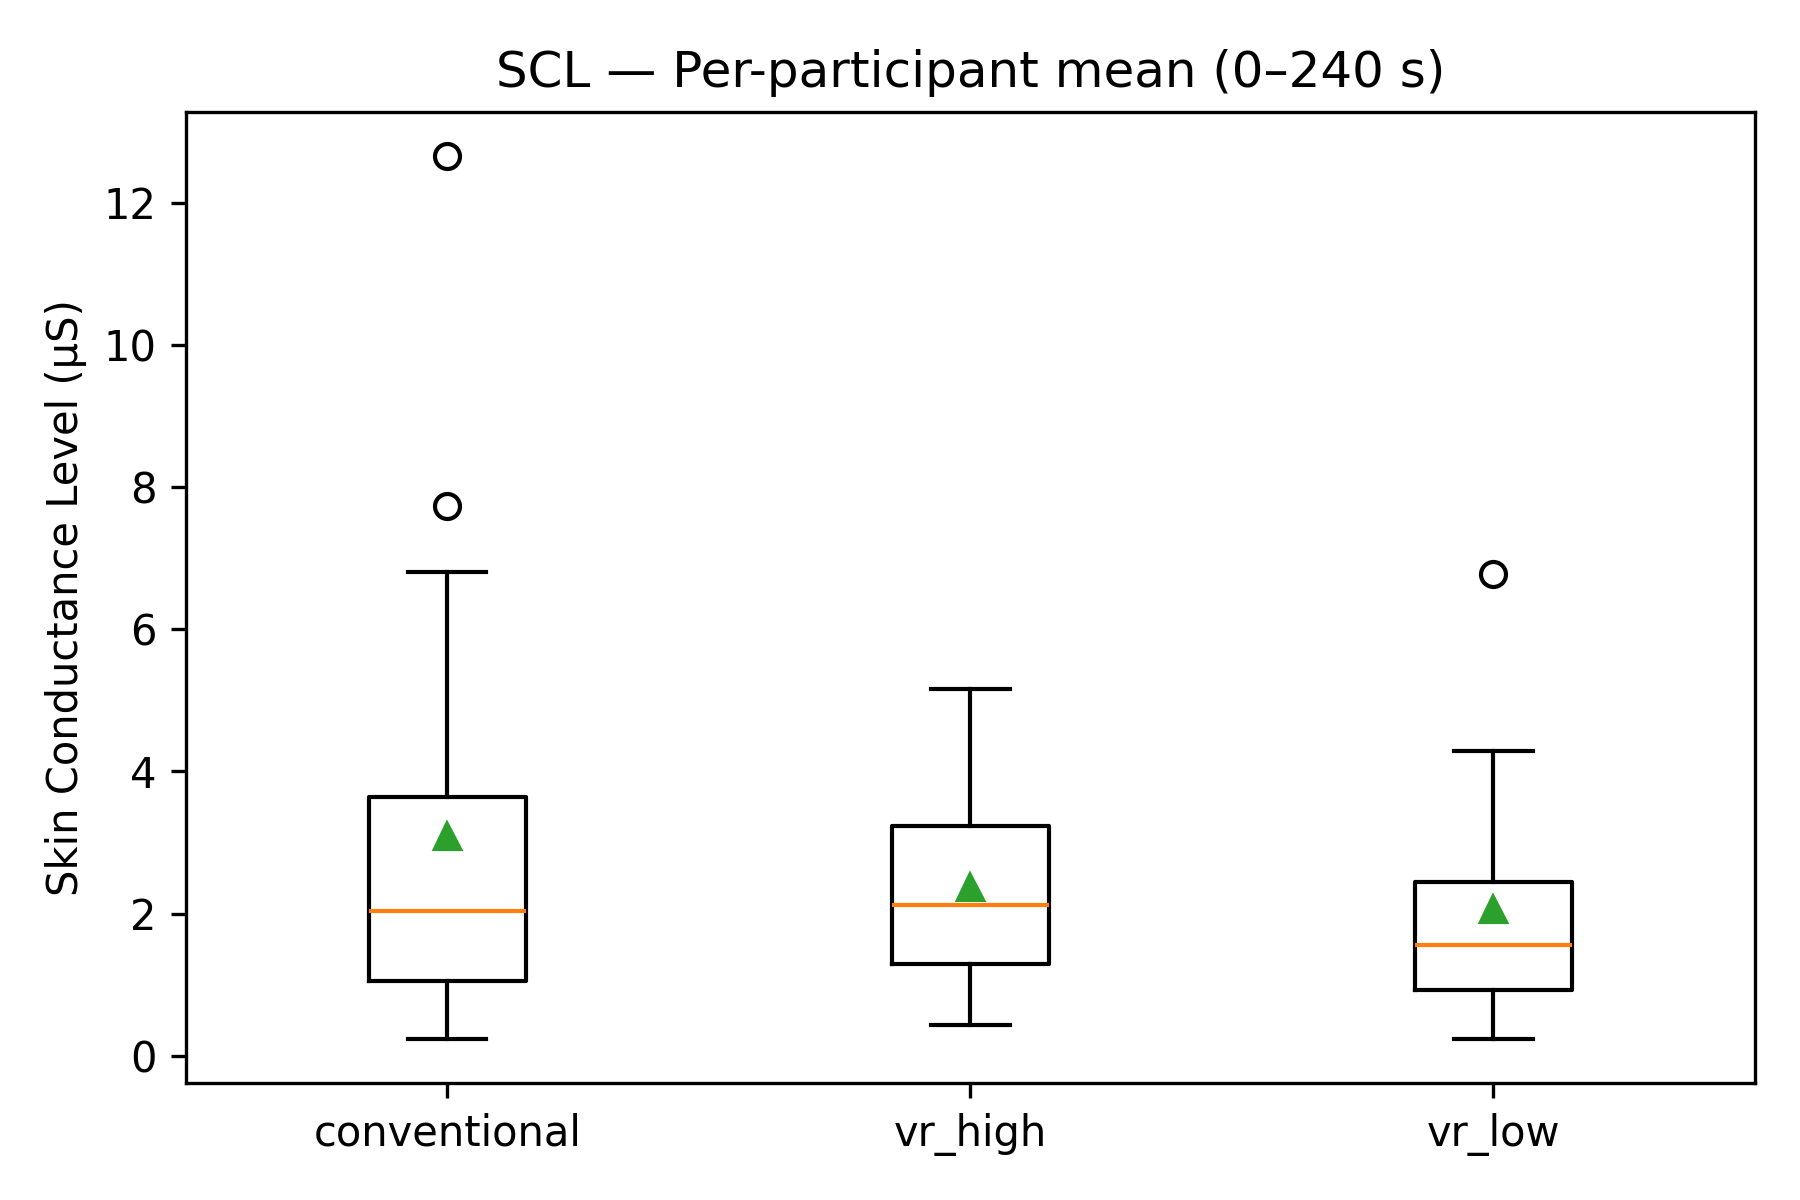
\includegraphics[width=\textwidth]{pics/result plots/boxplot_scl.png}
    \caption{Per-participant mean SCL during meditation (all three groups).}
    \label{fig:scl-perparticipant-supp}
\end{figure}

\begin{figure}[H]
    \centering
    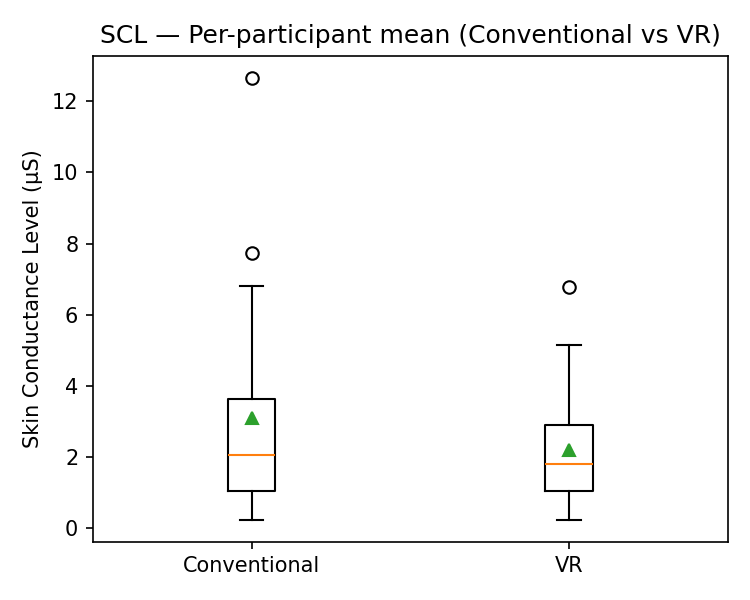
\includegraphics[width=\textwidth]{pics/result plots/box_collapsed_SCL.png}
    \caption{Per-participant mean SCL during meditation (Conventional vs.\ VR).}
    \label{fig:scl-perparticipant-convr}
\end{figure}

\begin{figure}[H]
    \centering
    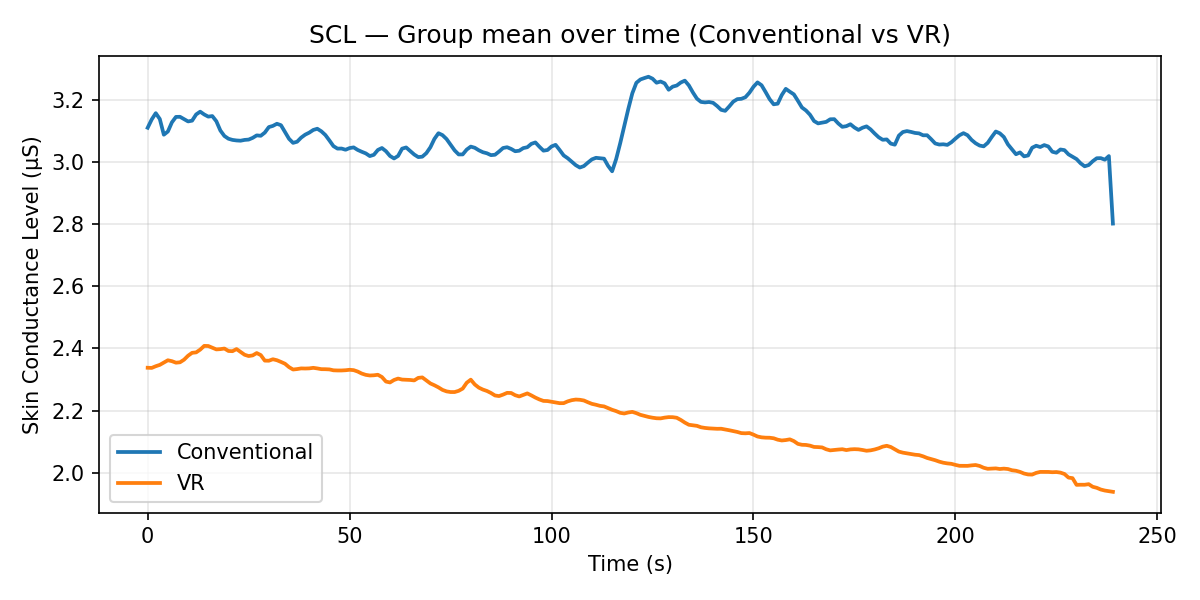
\includegraphics[width=\textwidth]{pics/result plots/lines_collapsed_SCL.png}
    \caption{Group-mean SCL over time for Conventional vs.\ VR.}
    \label{fig:scl-time-convr-supp}
\end{figure}

\section{Skin Temperature}

\begin{figure}[H]
    \centering
    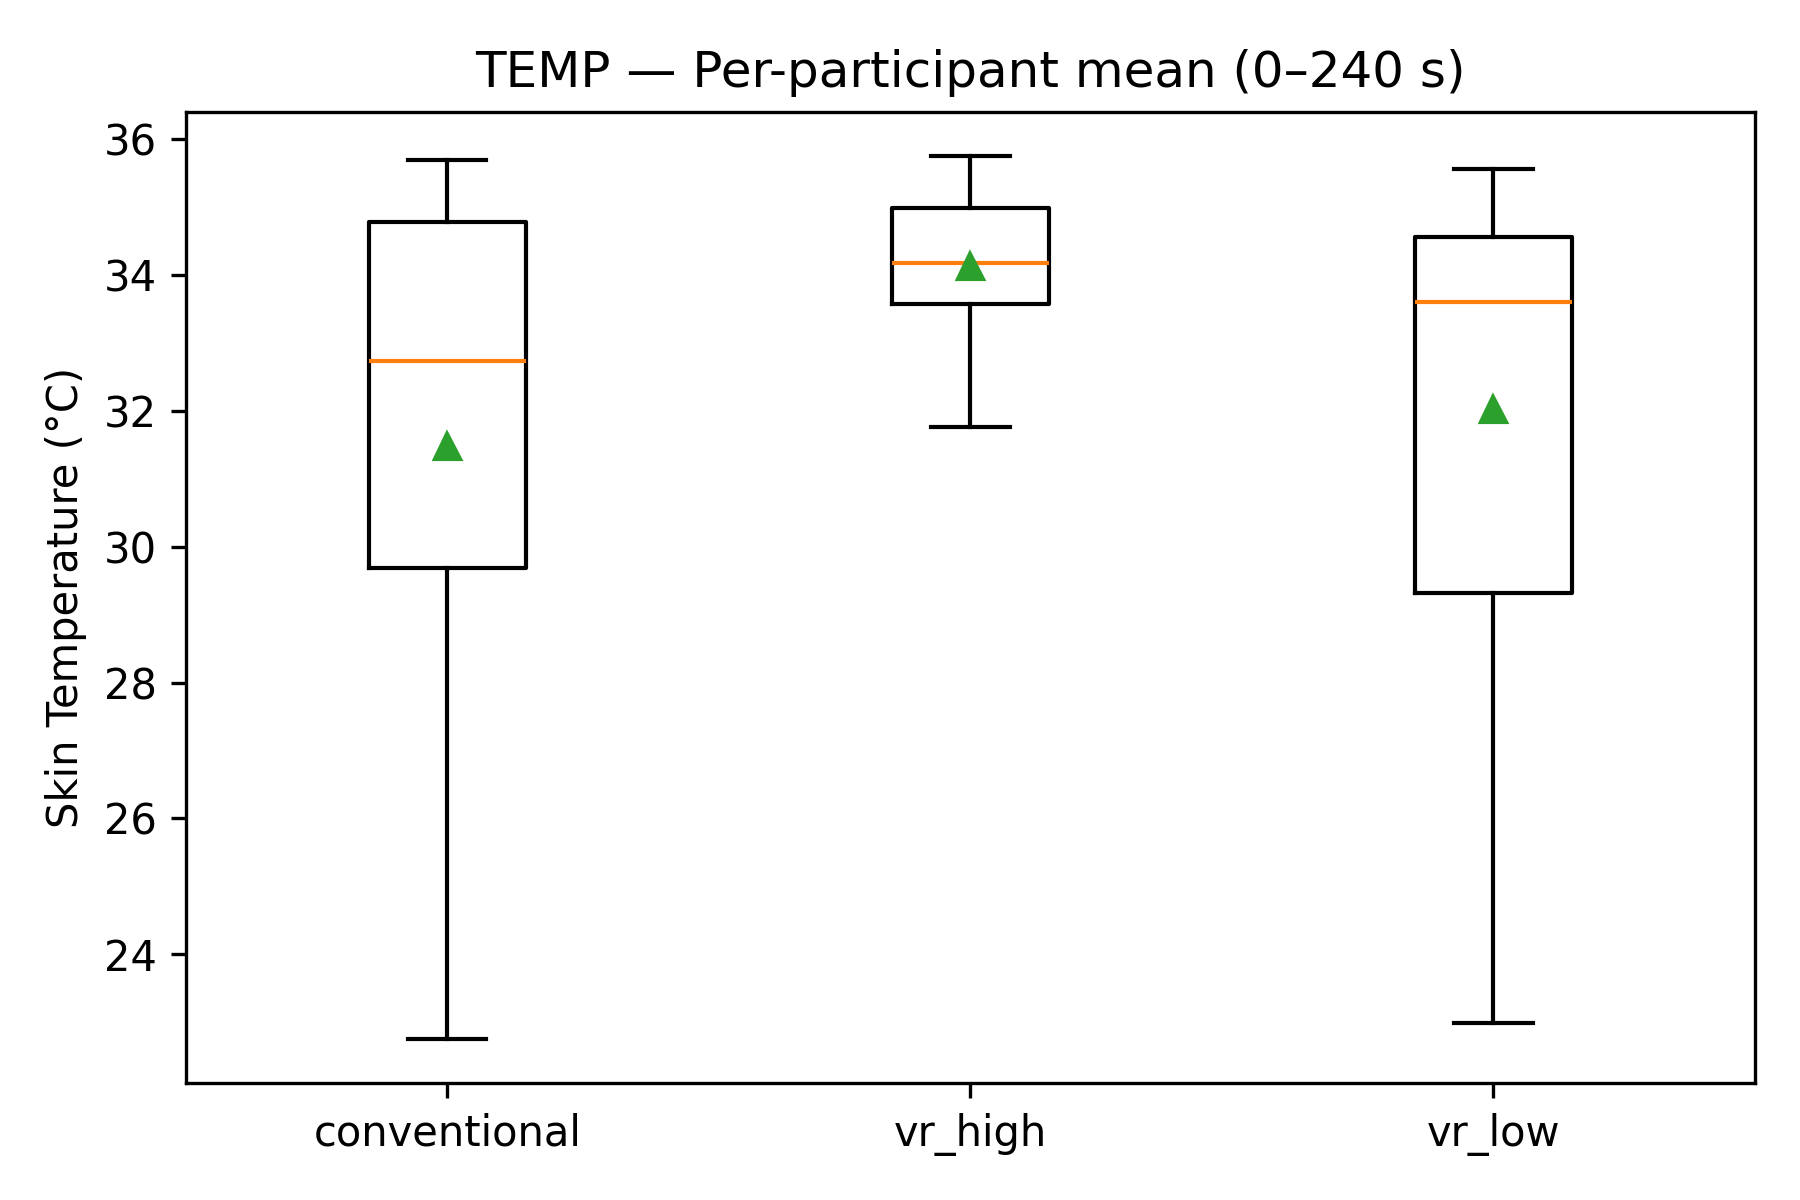
\includegraphics[width=\textwidth]{pics/result plots/boxplot_temp.png}
    \caption{Per-participant mean skin temperature during meditation (all three groups).}
    \label{fig:temp-perparticipant-supp}
\end{figure}

\begin{figure}[H]
    \centering
    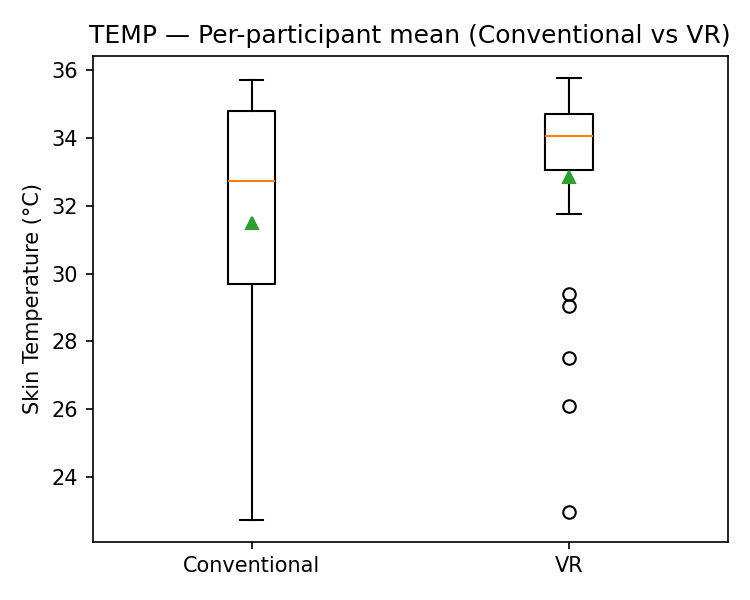
\includegraphics[width=\textwidth]{pics/result plots/box_collapsed_TEMP.png}
    \caption{Per-participant mean skin temperature (Conventional vs.\ VR).}
    \label{fig:temp-perparticipant-convr}
\end{figure}

\begin{figure}[H]
    \centering
    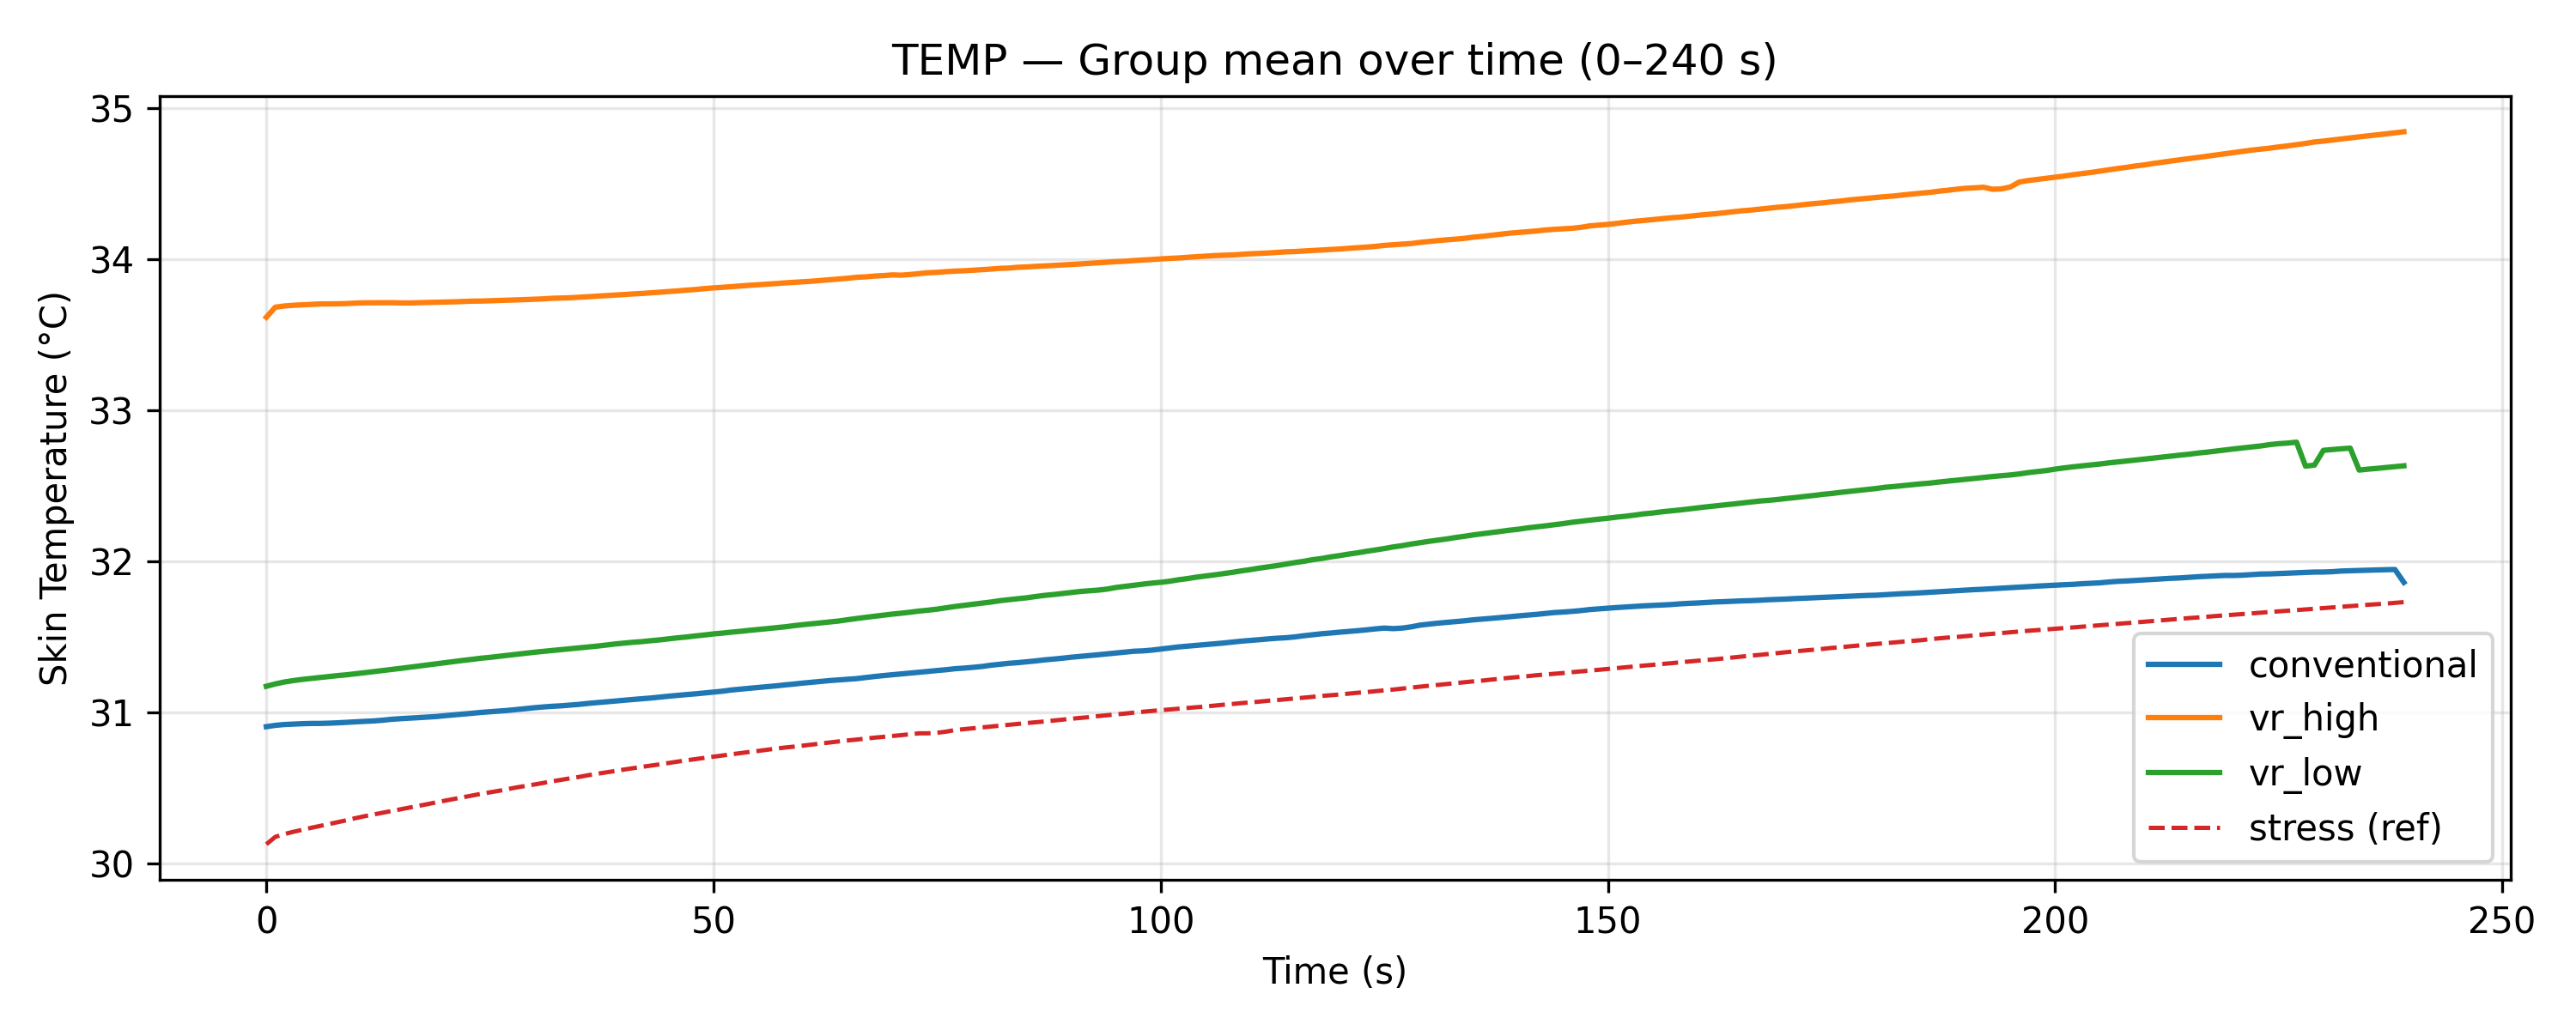
\includegraphics[width=\textwidth]{pics/result plots/timeseries_temp.png}
    \caption{Group-mean skin temperature over time for all three groups.}
    \label{fig:temp-time-supp}
\end{figure}

\section{Pulse Volume Amplitude (PVA)}

\begin{figure}[H]
    \centering
    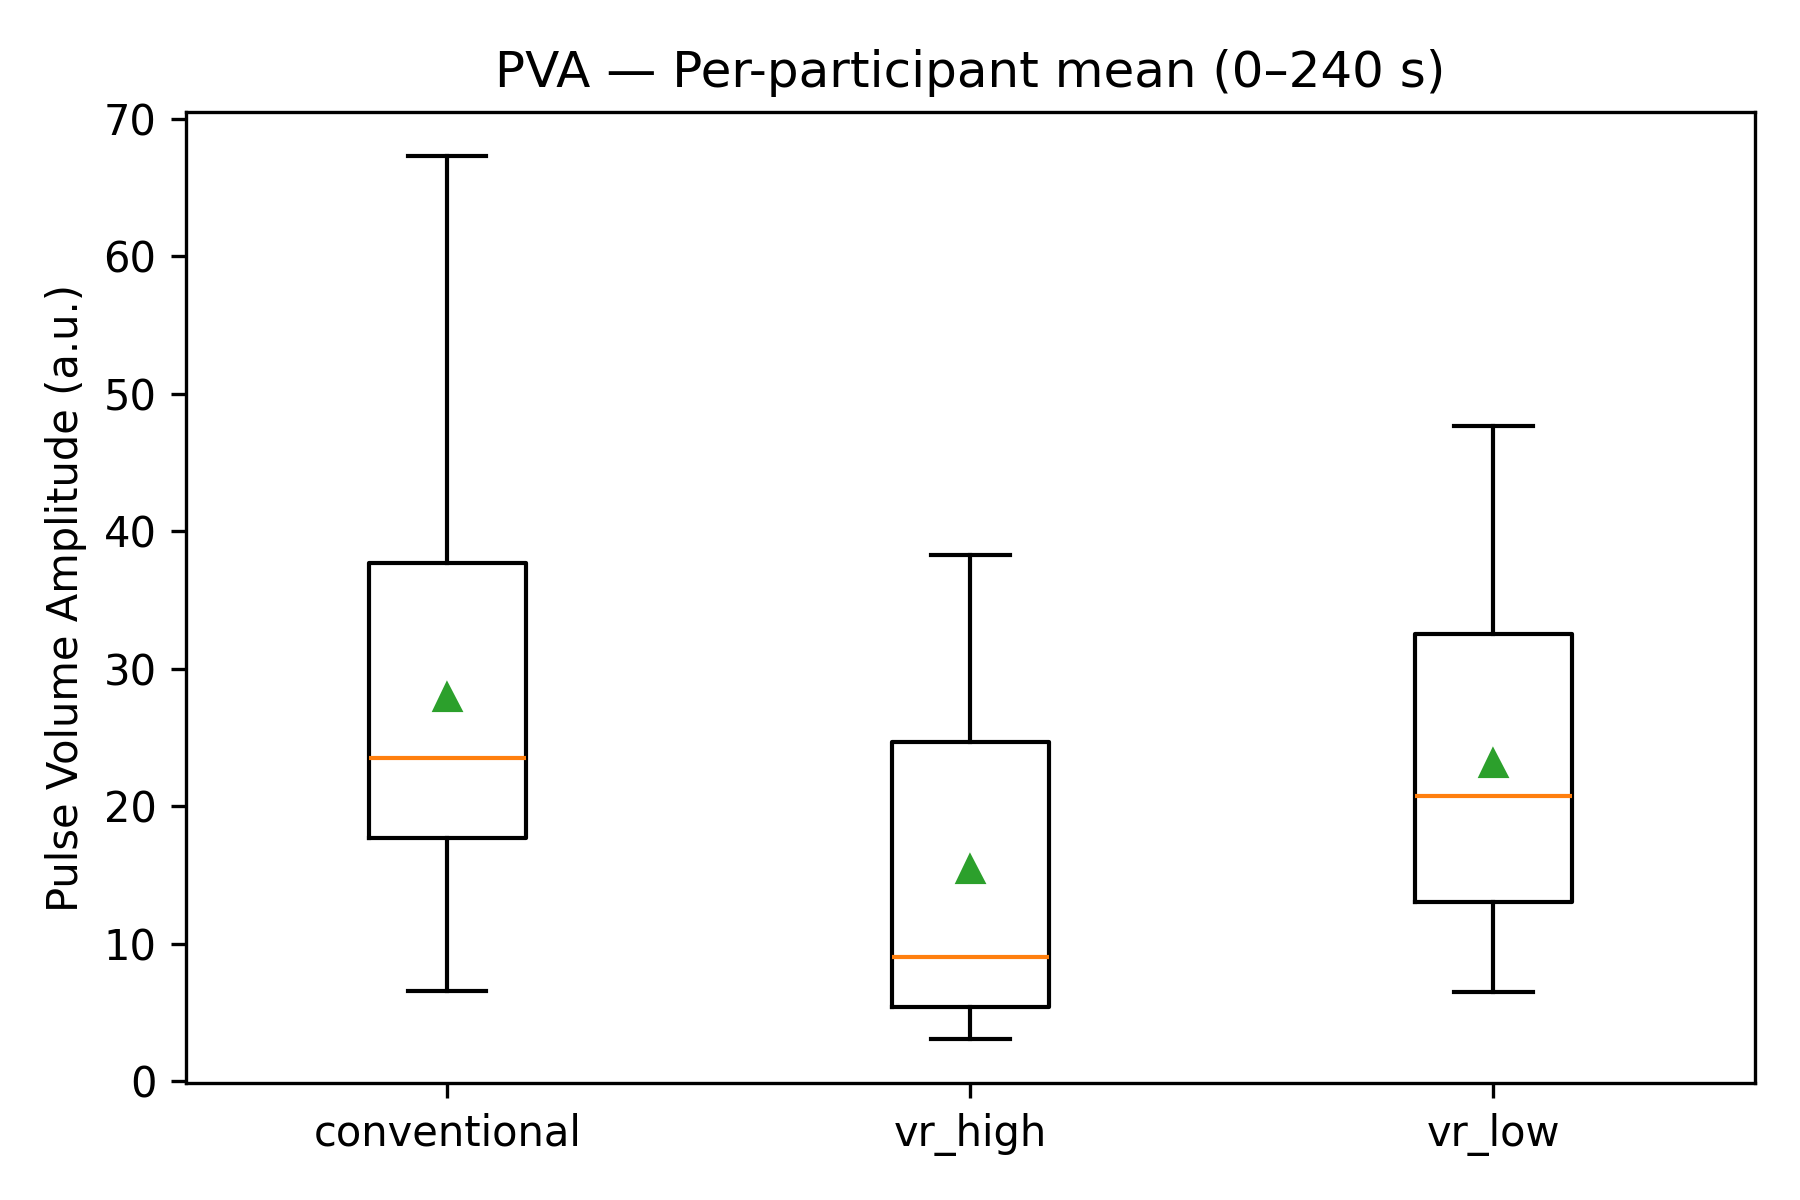
\includegraphics[width=\textwidth]{pics/result plots/boxplot_pva.png}
    \caption{Per-participant mean PVA during meditation (all three groups).}
    \label{fig:pva-perparticipant-supp}
\end{figure}

\begin{figure}[H]
    \centering
    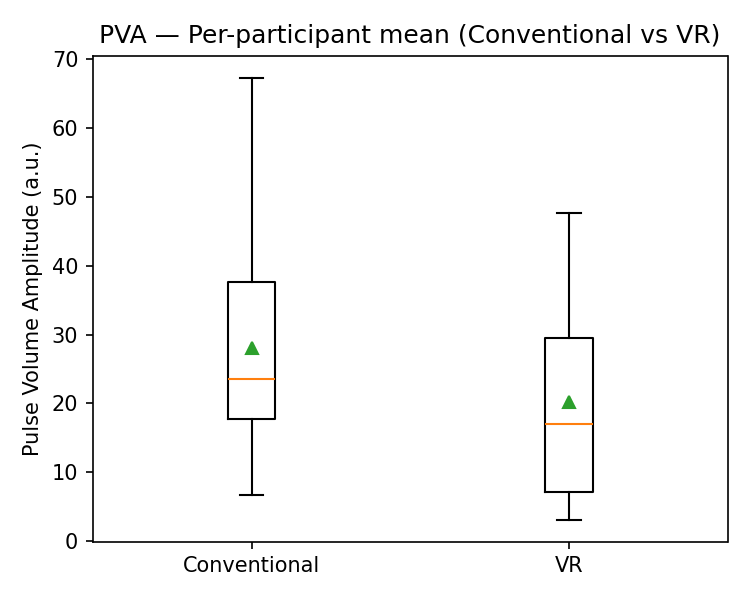
\includegraphics[width=\textwidth]{pics/result plots/box_collapsed_PVA.png}
    \caption{Per-participant mean PVA (Conventional vs.\ VR).}
    \label{fig:pva-perparticipant-convr}
\end{figure}

\begin{figure}[H]
    \centering
    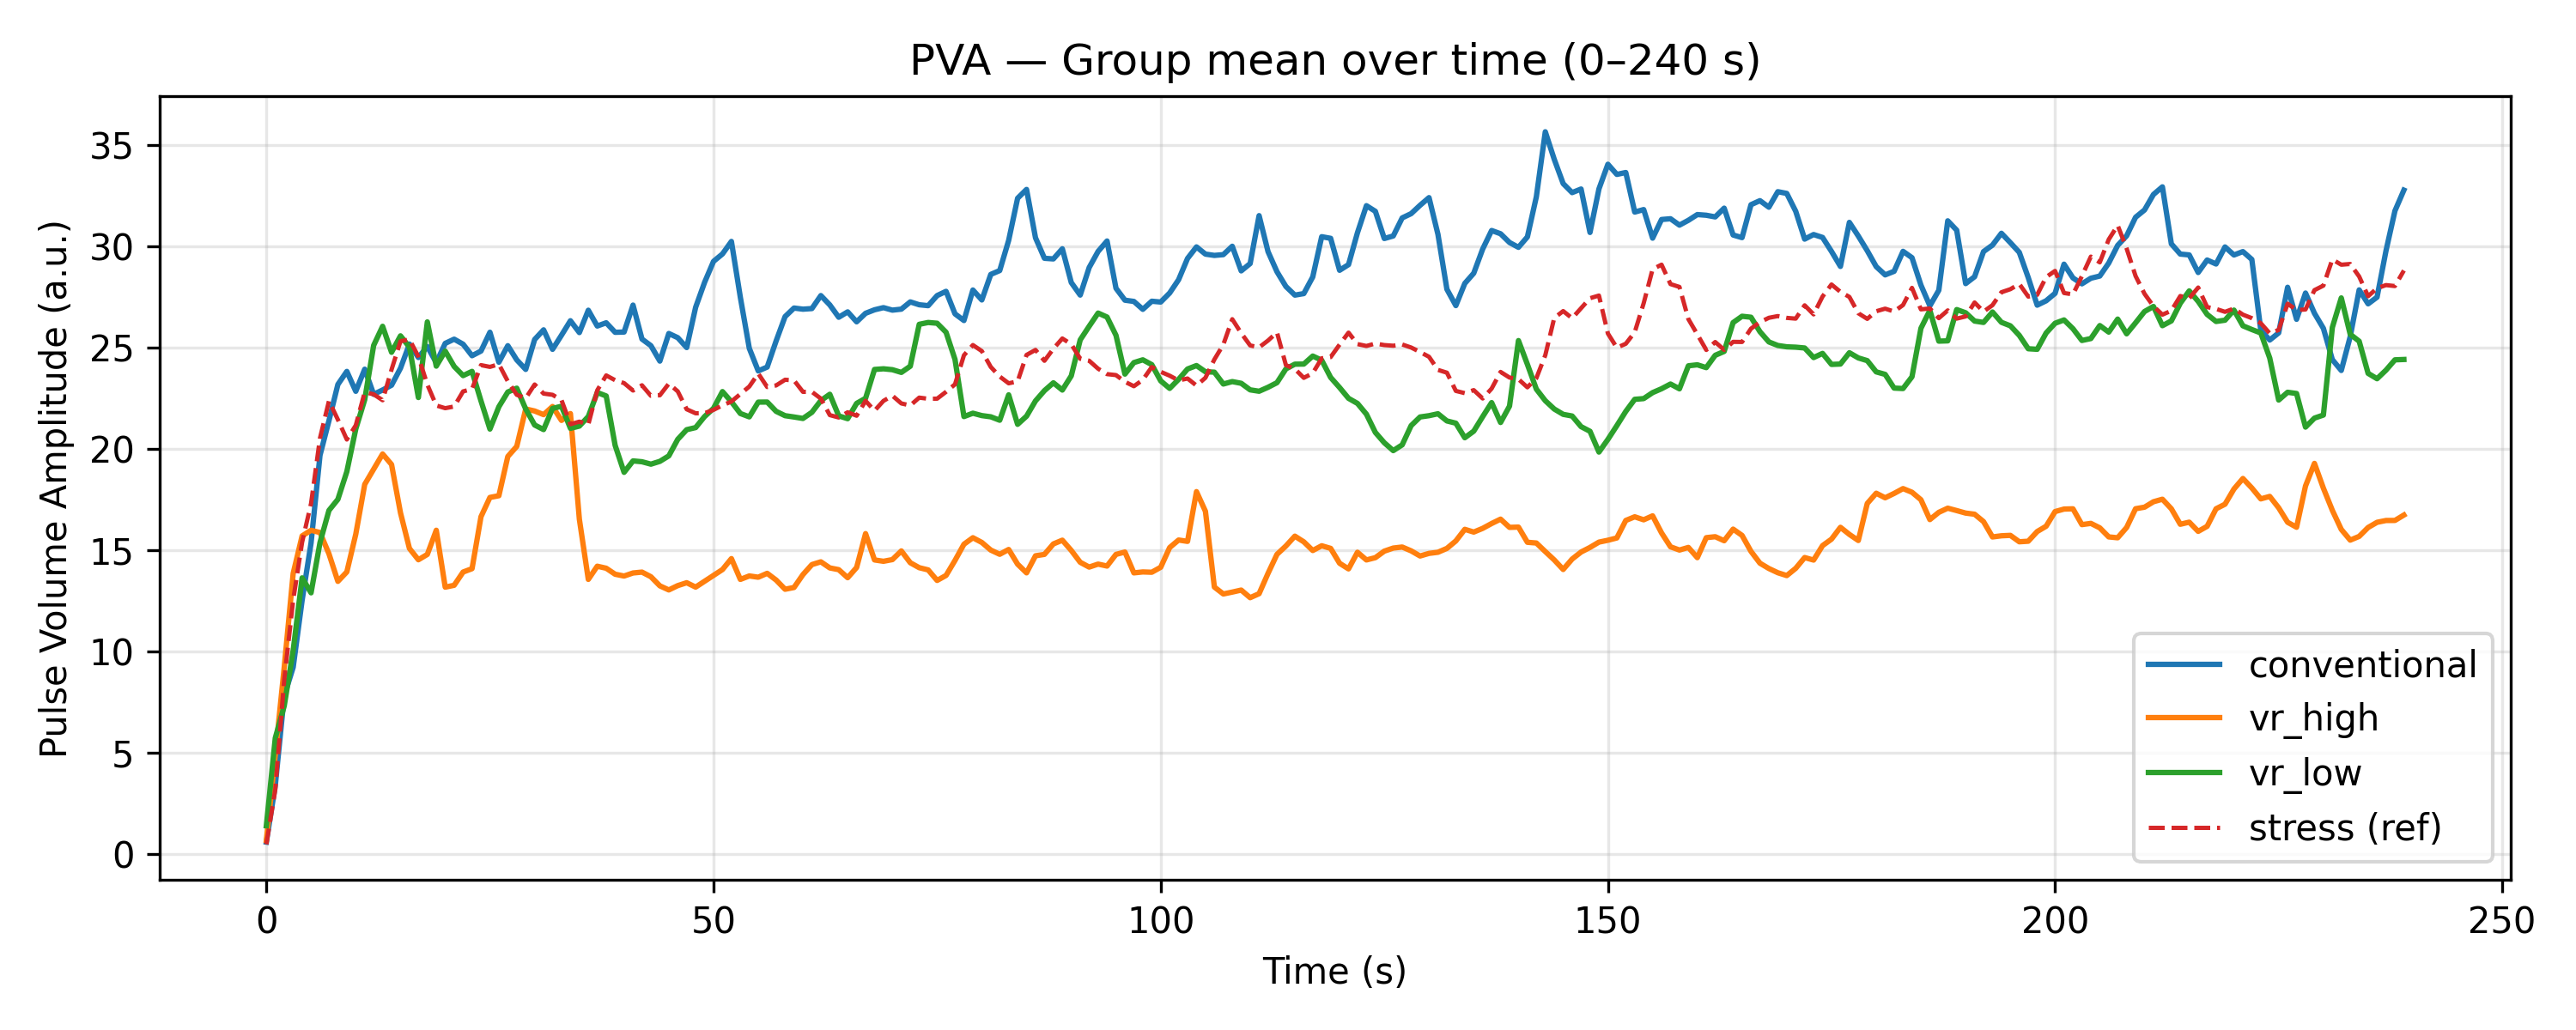
\includegraphics[width=\textwidth]{pics/result plots/timeseries_pva.png}
    \caption{Group-mean PVA over time  for all three groups.}
    \label{fig:pva-time-supp}
\end{figure}

\begin{figure}[H]
    \centering
    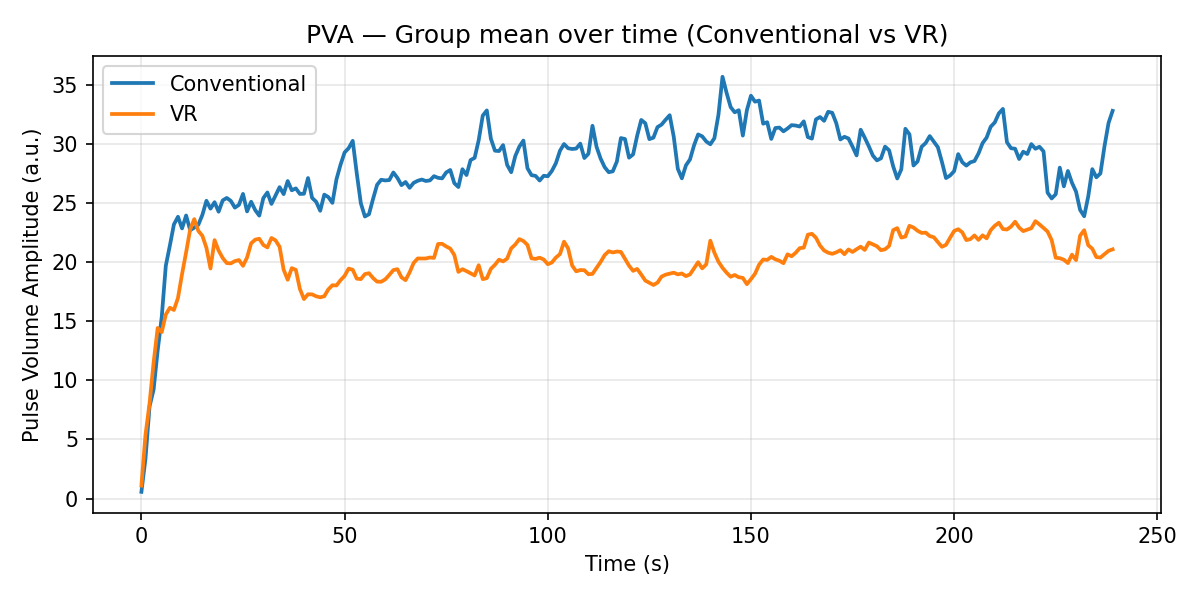
\includegraphics[width=\textwidth]{pics/result plots/lines_collapsed_PVA.png}
    \caption{Group-mean PVA over time (Conventional vs.\ VR).}
    \label{fig:pva-time-convr}
\end{figure}

\section{Body Motion}

\begin{figure}[H]
    \centering
    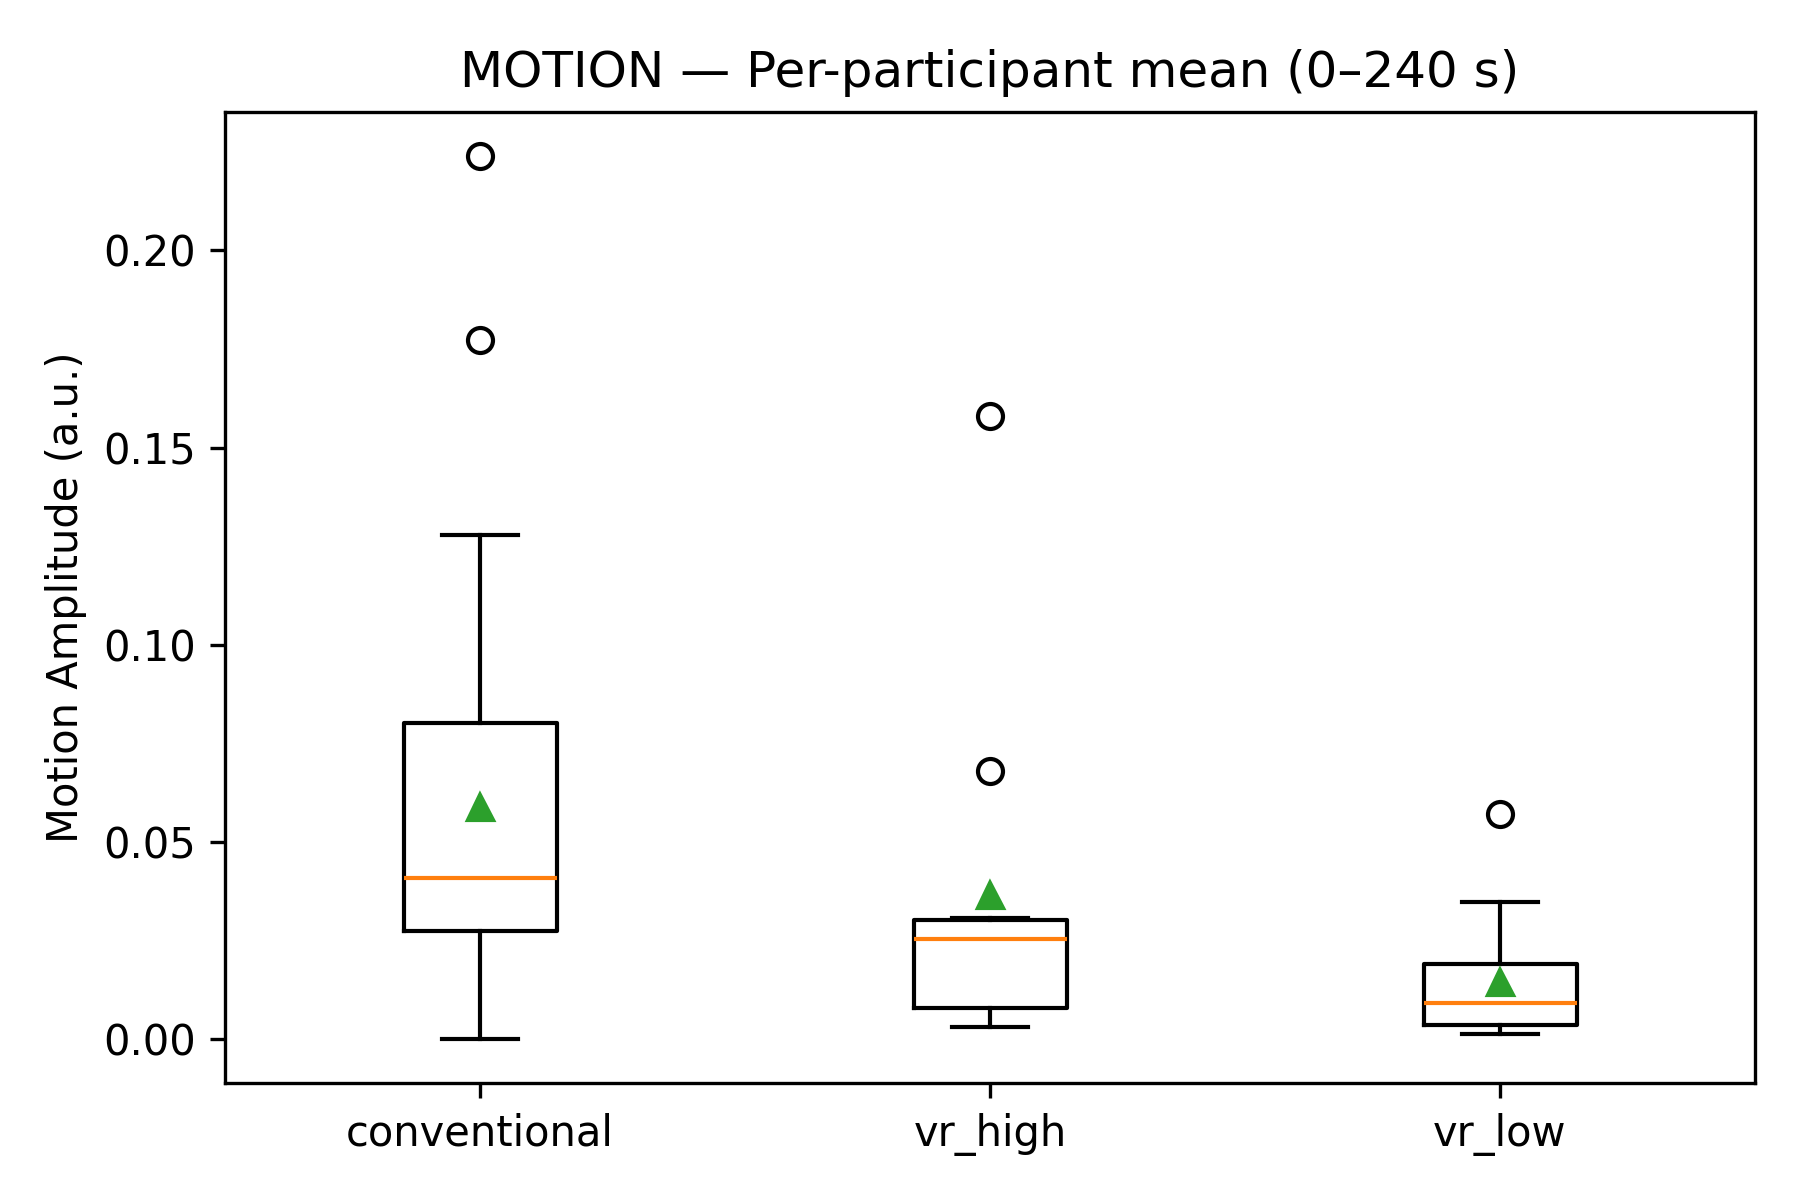
\includegraphics[width=\textwidth]{pics/result plots/boxplot_motion.png}
    \caption{Per-participant mean motion amplitude during meditation (all three groups).}
    \label{fig:motion-perparticipant-supp}
\end{figure}

\begin{figure}[H]
    \centering
    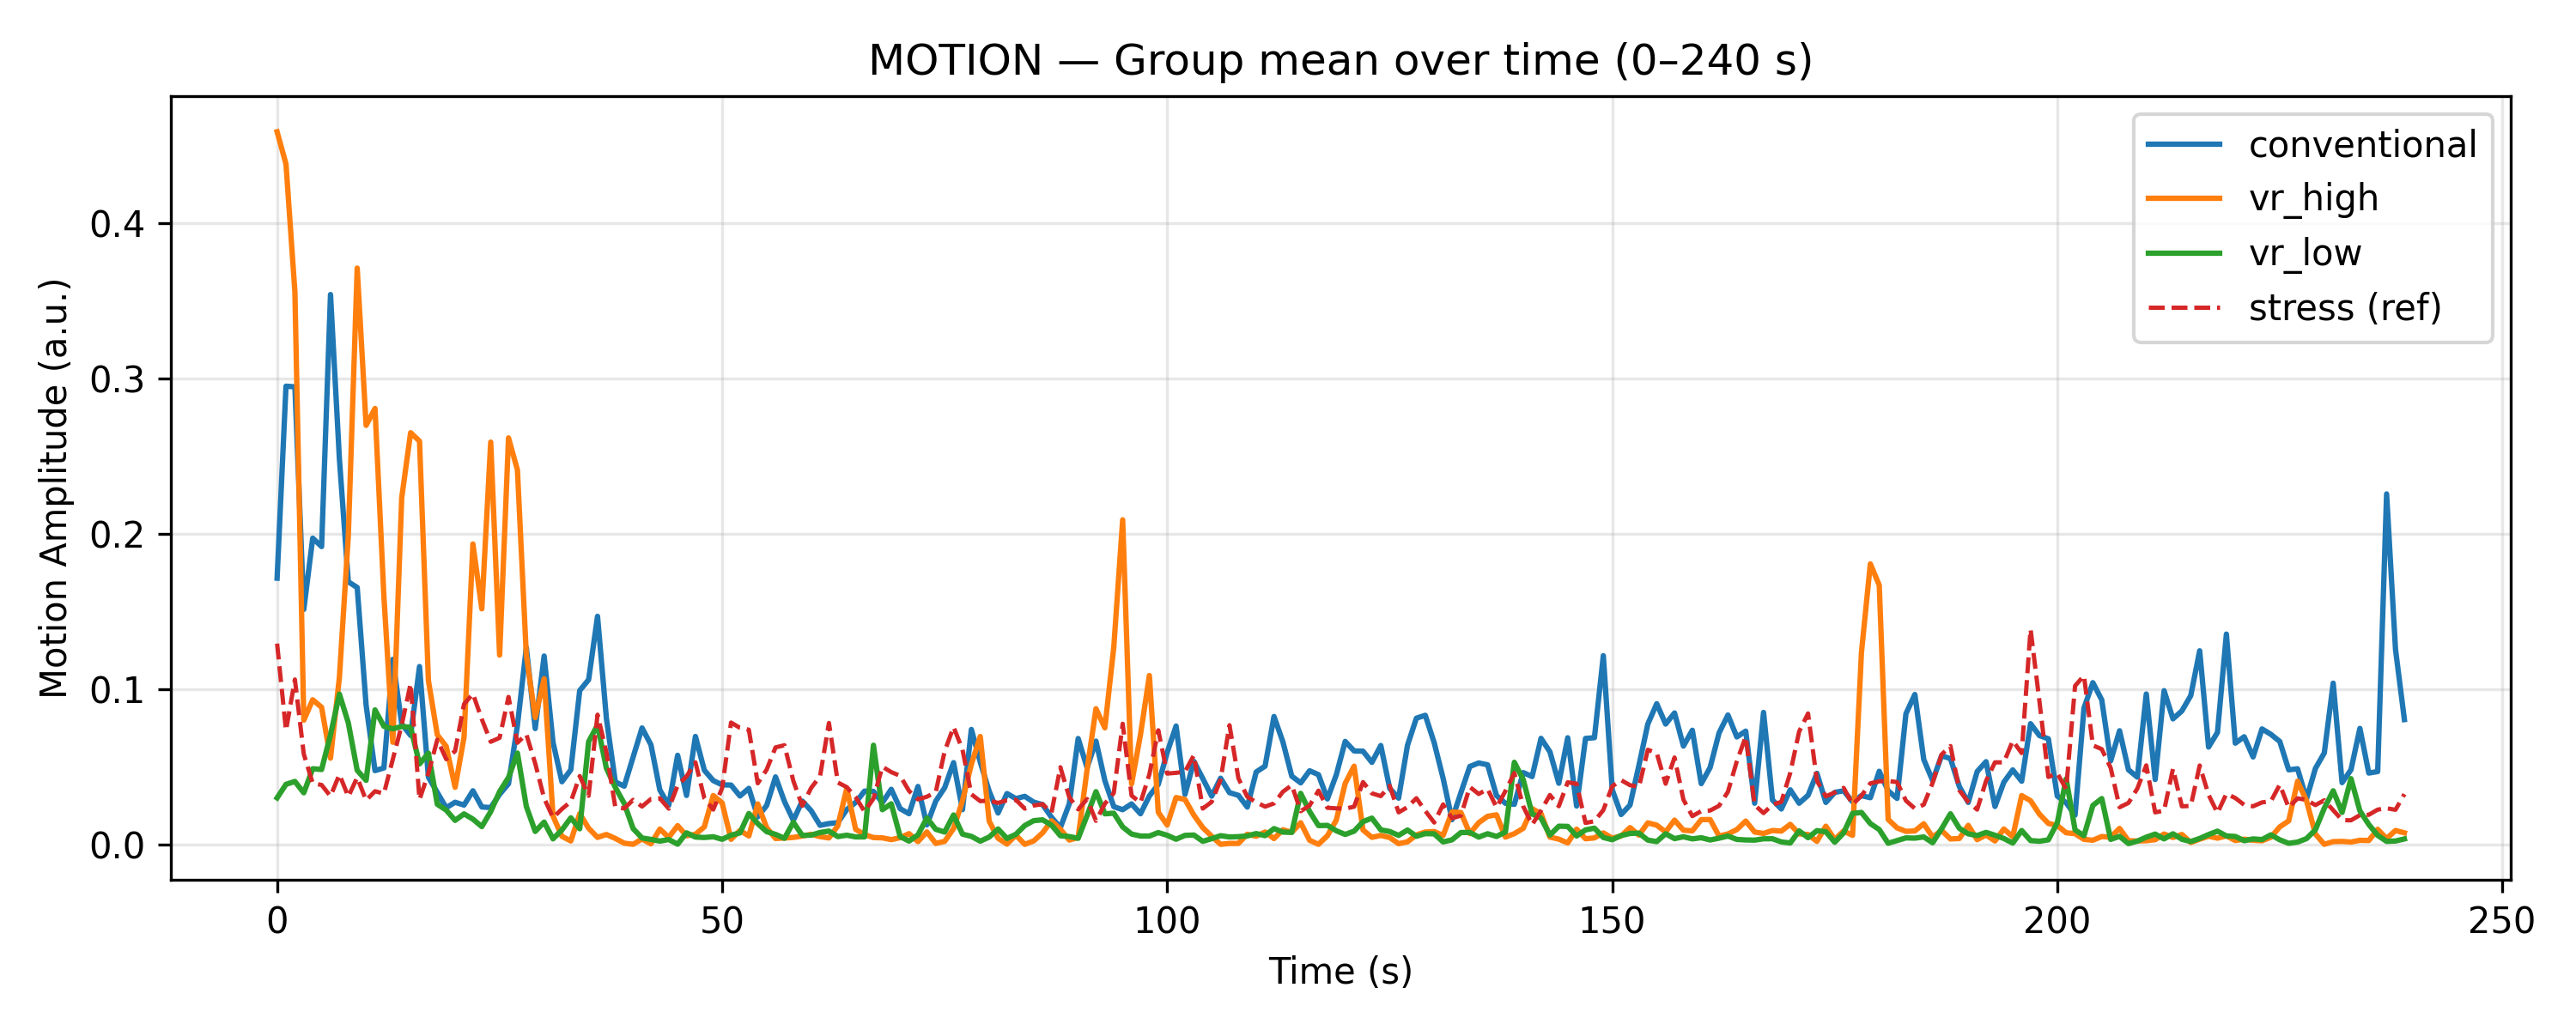
\includegraphics[width=\textwidth]{pics/result plots/timeseries_motion.png}
    \caption{Group-mean motion amplitude over time for all three groups.}
    \label{fig:motion-time-supp}
\end{figure}

\begin{figure}[H]
    \centering
    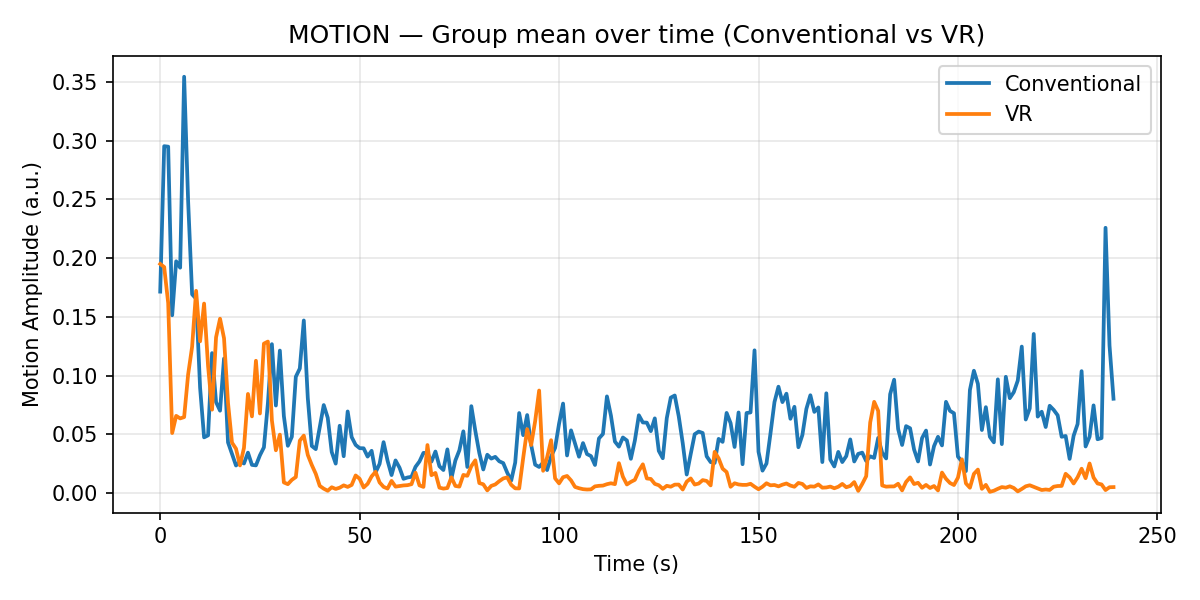
\includegraphics[width=\textwidth]{pics/result plots/lines_collapsed_MOTION.png}
    \caption{Group-mean motion amplitude over time (Conventional vs.\ VR).}
    \label{fig:motion-time-convr}
\end{figure}

\section{Additional HRV Visualisations}

\begin{figure}[H]
    \centering
    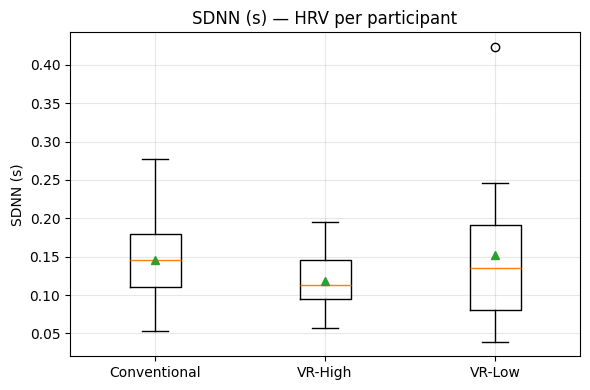
\includegraphics[width=\textwidth]{pics/result plots/new result comparison/SDNN per participant.png}
    \caption{Per-participant SDNN across groups.}
    \label{fig:sdnn-supp}
\end{figure}

\begin{figure}[H]
    \centering
    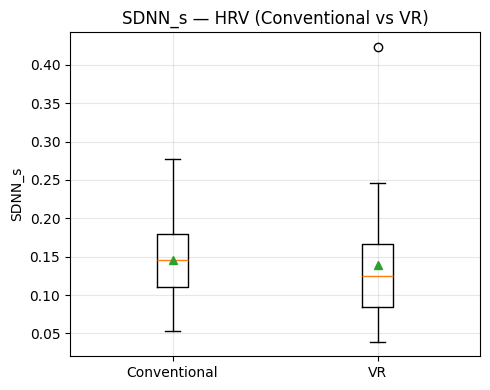
\includegraphics[width=\textwidth]{pics/comparison/SDNN_s-HRV (Con bs VR).png}
    \caption{SDNN comparison between Conventional and VR.}
    \label{fig:sdnn-convr-supp}
\end{figure}

\begin{figure}[H]
    \centering
    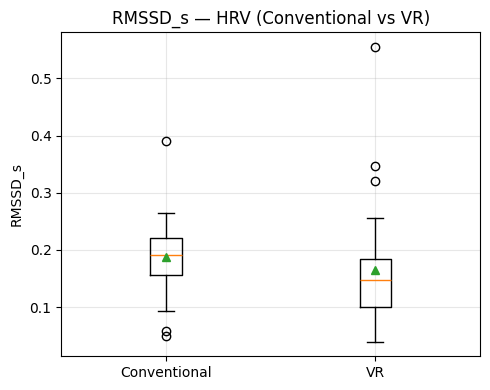
\includegraphics[width=\textwidth]{pics/comparison/RMSSD_s-HRV(con vs VR).png}
    \caption{RMSSD comparison between Conventional and VR.}
    \label{fig:rmssd-convr-supp}
\end{figure}
\begin{figure}[H]
    \centering
    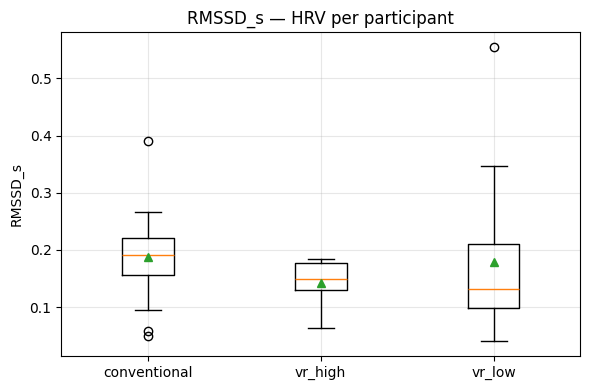
\includegraphics[width=\textwidth]{pics/comparison/RMSSD_s-HRV per participant.png}
    \caption{RMSSD comparison between 3 groups.}
    \label{fig:rmssd-convr-supp}
\end{figure}


\begin{figure}[H]
    \centering
    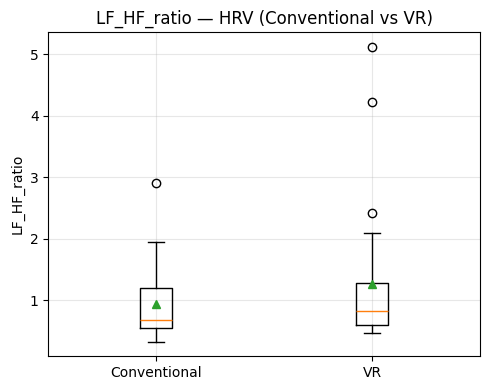
\includegraphics[width=\textwidth]{pics/comparison/LF-HR ratio-HRV(con vs VR).png}
    \caption{LF/HF ratio comparison between Conventional and VR.}
    \label{fig:lfhf-convr-supp}
\end{figure}



\begin{figure}[t]
  \centering
  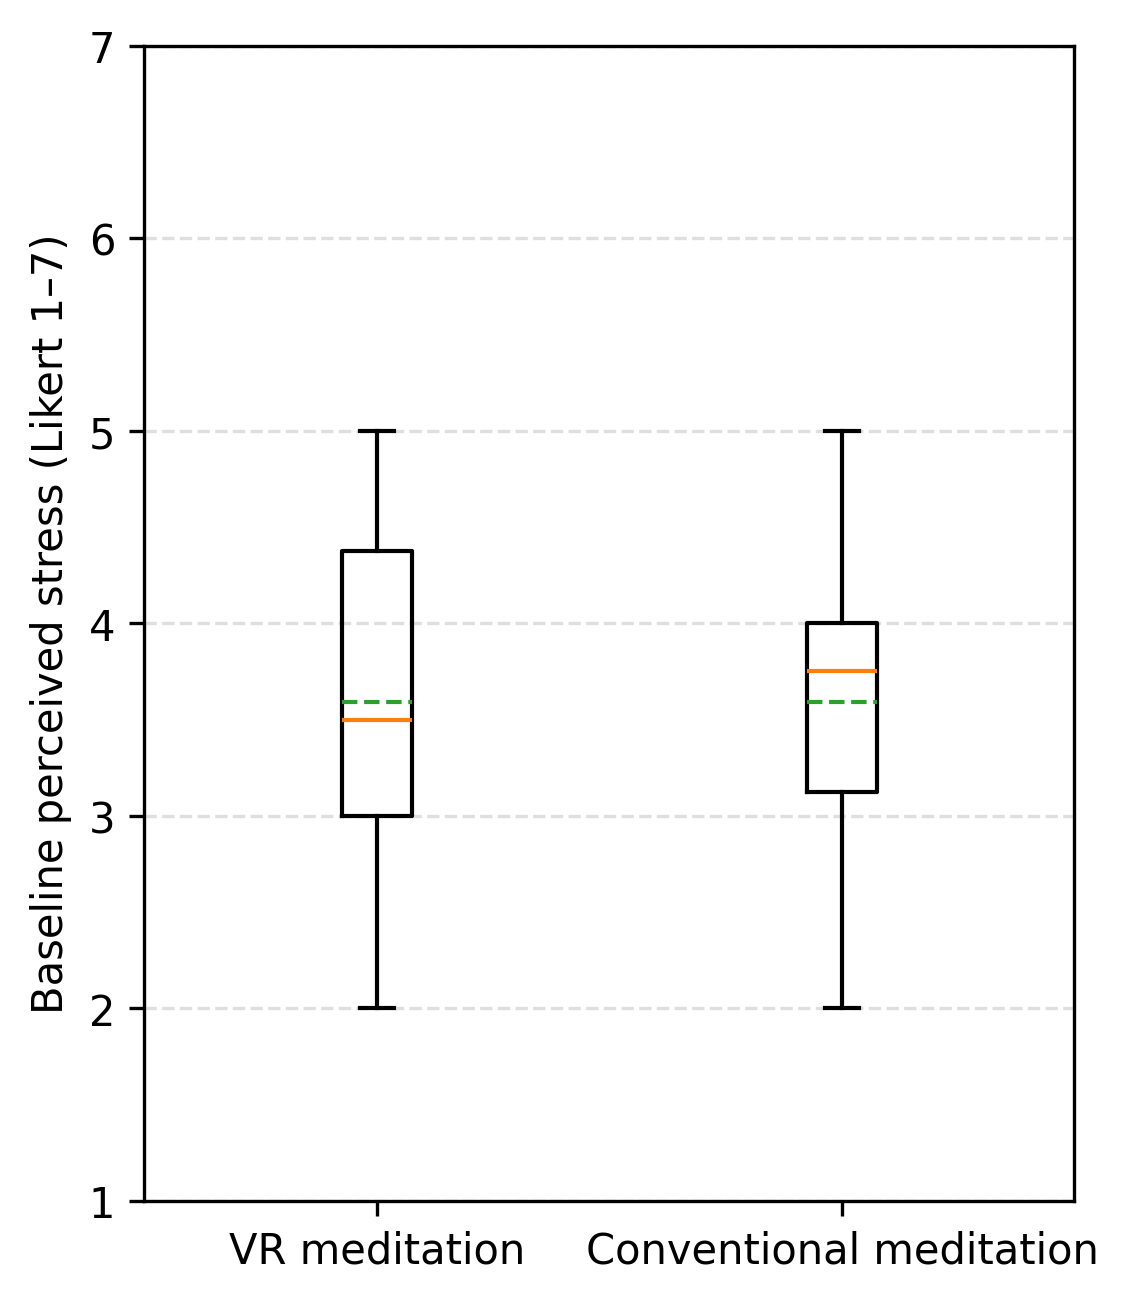
\includegraphics[width=.55\textwidth]{pics/fig1_stress_score_VR_vs_Conventional.png}
  \caption[Baseline perceived stress by mode of delivery]%
  {Baseline perceived stress ratings for VR and conventional meditation.
   Boxplots show median, interquartile range, and whiskers
   (1.5~$\times$~IQR); the dashed line indicates the group mean.}
  \label{fig:stress_questionnaire}
\end{figure}

\begin{figure}[t]
  \centering
  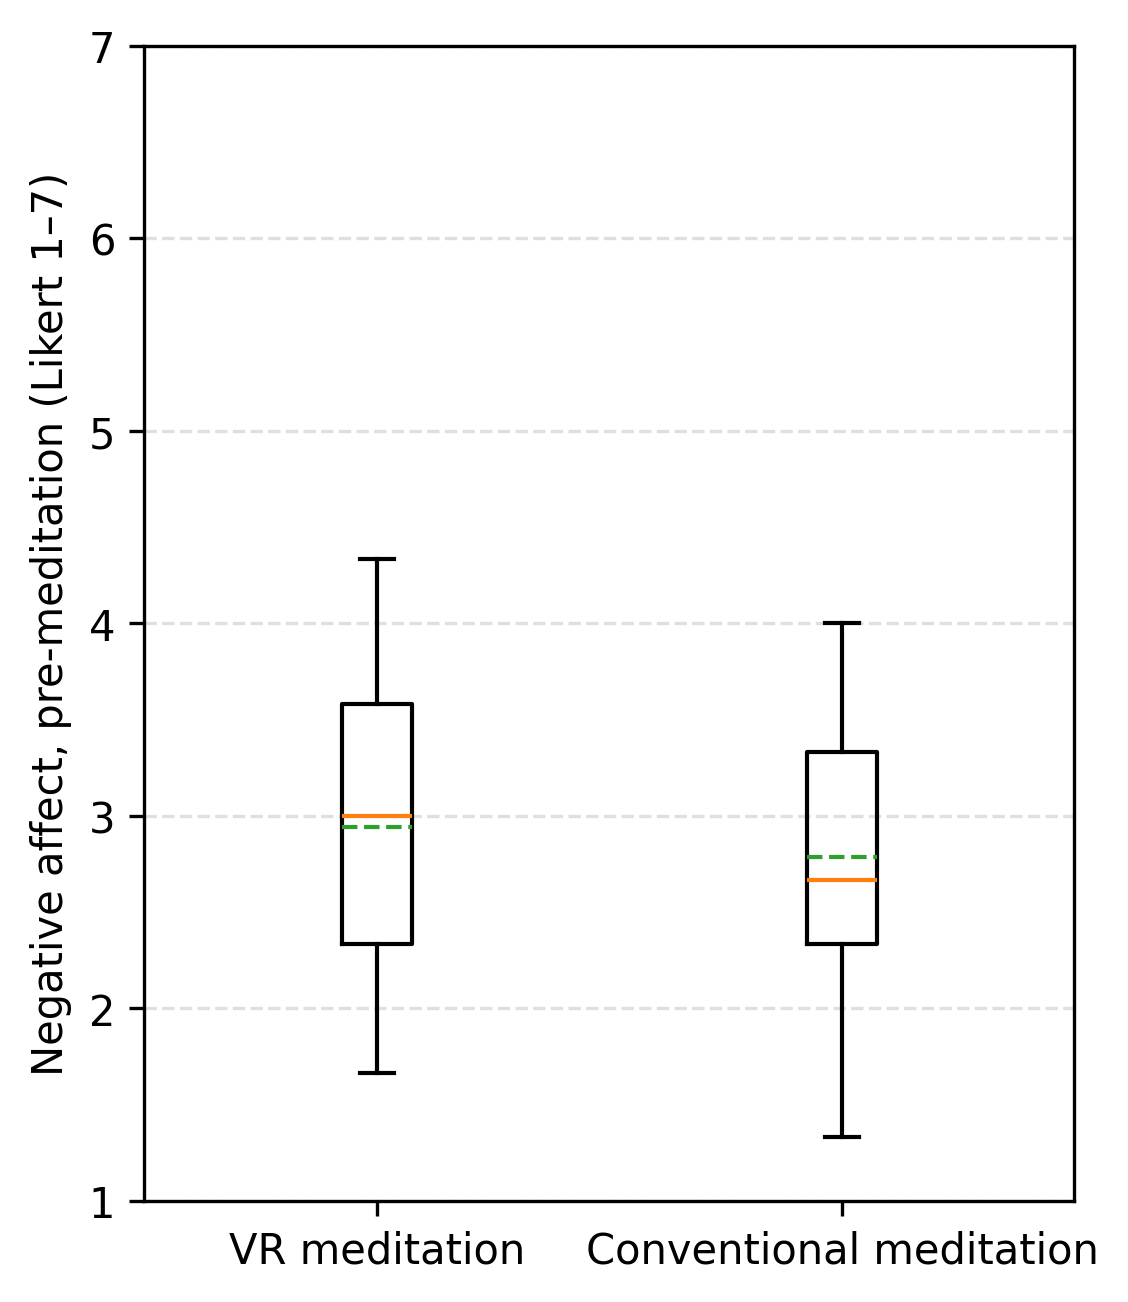
\includegraphics[width=.55\textwidth]{pics/fig2_affect_pre_neg_VR_vs_Conventional.png}
  \caption[Negative affect before meditation by mode of delivery]%
  {Negative affect ratings before the meditation session for VR and
   conventional meditation.}
  \label{fig:affect_pre_questionnaire}
\end{figure}



\begin{figure}[t]
  \centering
  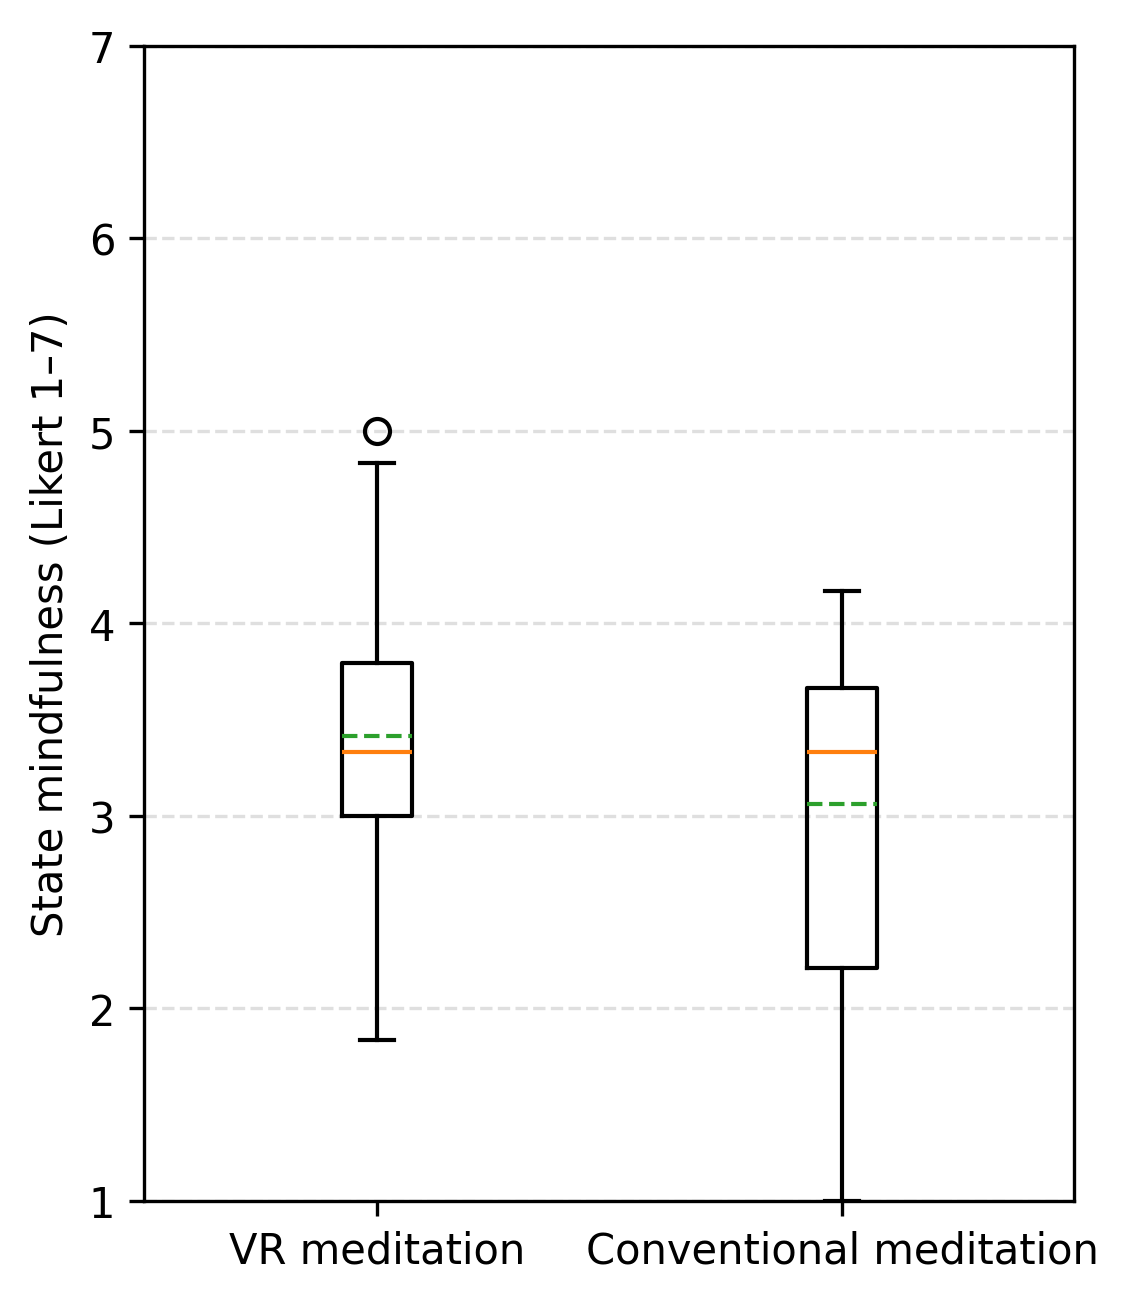
\includegraphics[width=.55\textwidth]{pics/fig3_mindfulness_VR_vs_Conventional.png}
  \caption[State mindfulness by mode of delivery]%
  {State mindfulness ratings during meditation for VR and conventional
   conditions.}
  \label{fig:mindfulness_questionnaire}
\end{figure}

\begin{figure}[t]
  \centering
  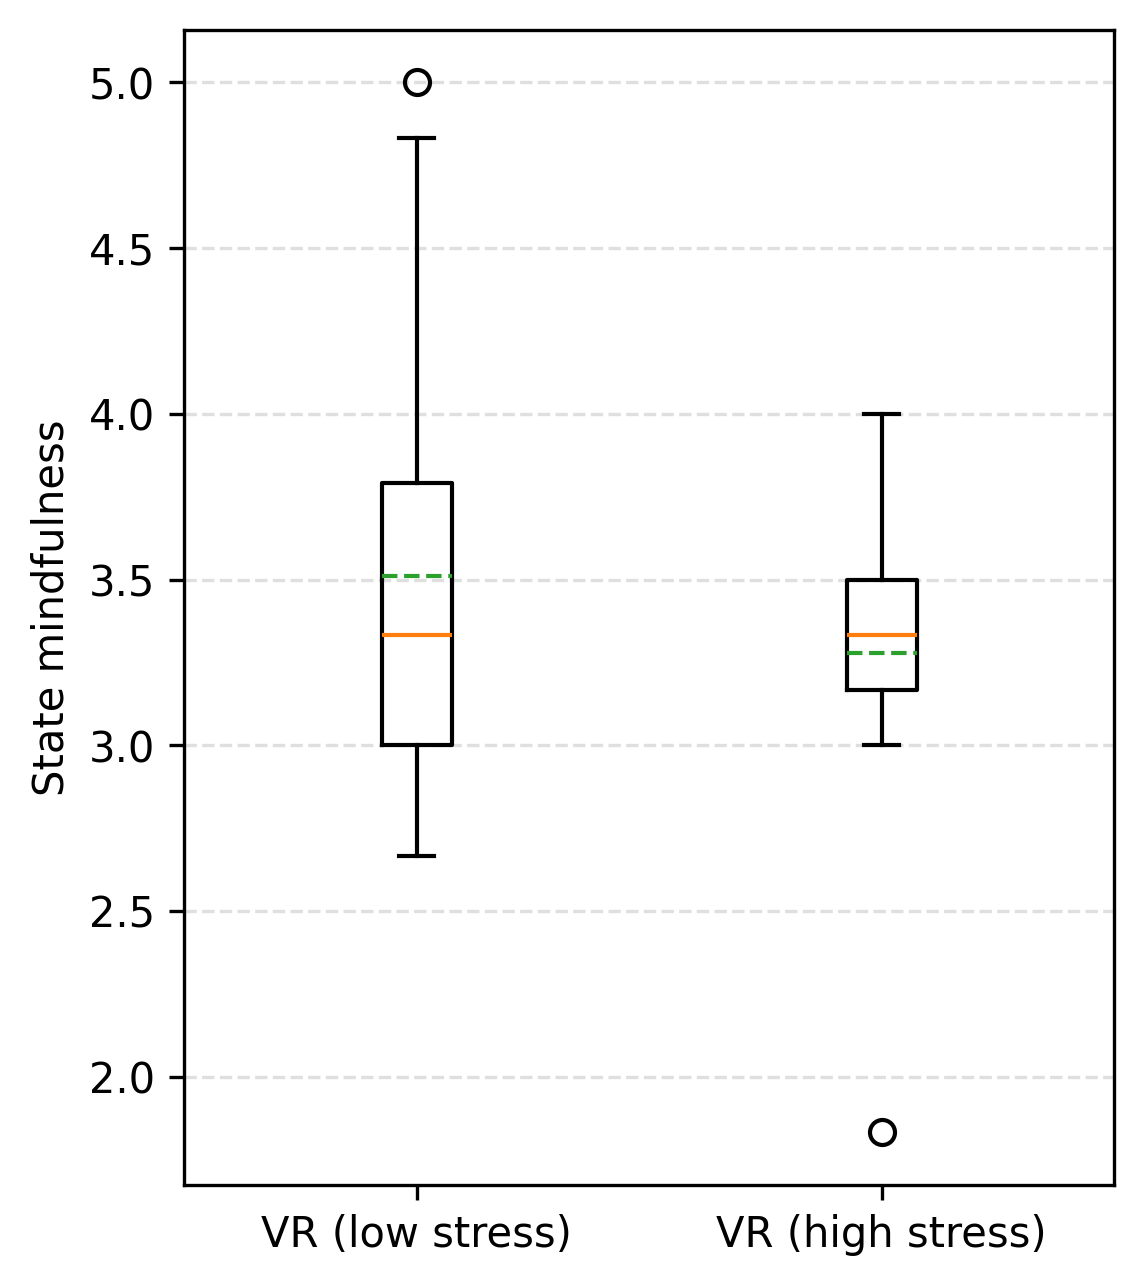
\includegraphics[width=.55\textwidth]{pics/fig6_mindfulness_vr_low_vs_vr_high.png}
  \caption[State mindfulness in VR low- vs.\ high-stress subgroups]%
  {State mindfulness ratings for VR participants with low vs.\ high
   physiological stress.}
  \label{fig:mindfulness_vr_subgroups}
\end{figure}

\begin{figure}[t]
  \centering
  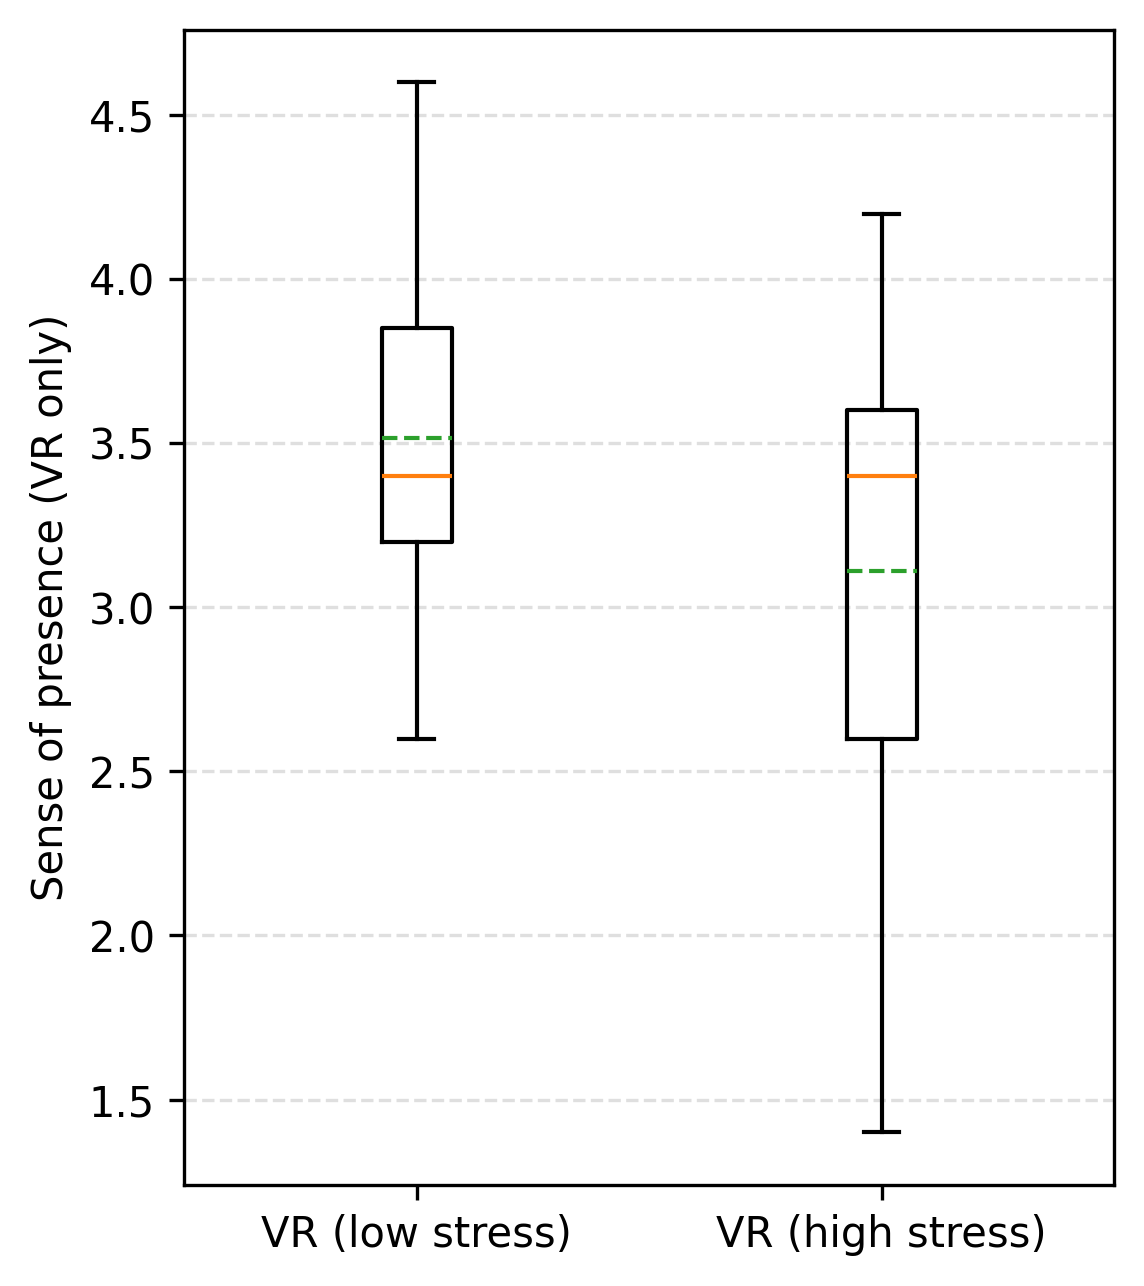
\includegraphics[width=.55\textwidth]{pics/fig7_presence_vr_low_vs_vr_high.png}
  \caption[Presence in VR low- vs.\ high-stress subgroups]%
  {Sense of presence for VR participants in the low- and high-stress
   subgroups.}
  \label{fig:presence_vr_subgroups}
\end{figure}

\begin{figure}[t]
  \centering
  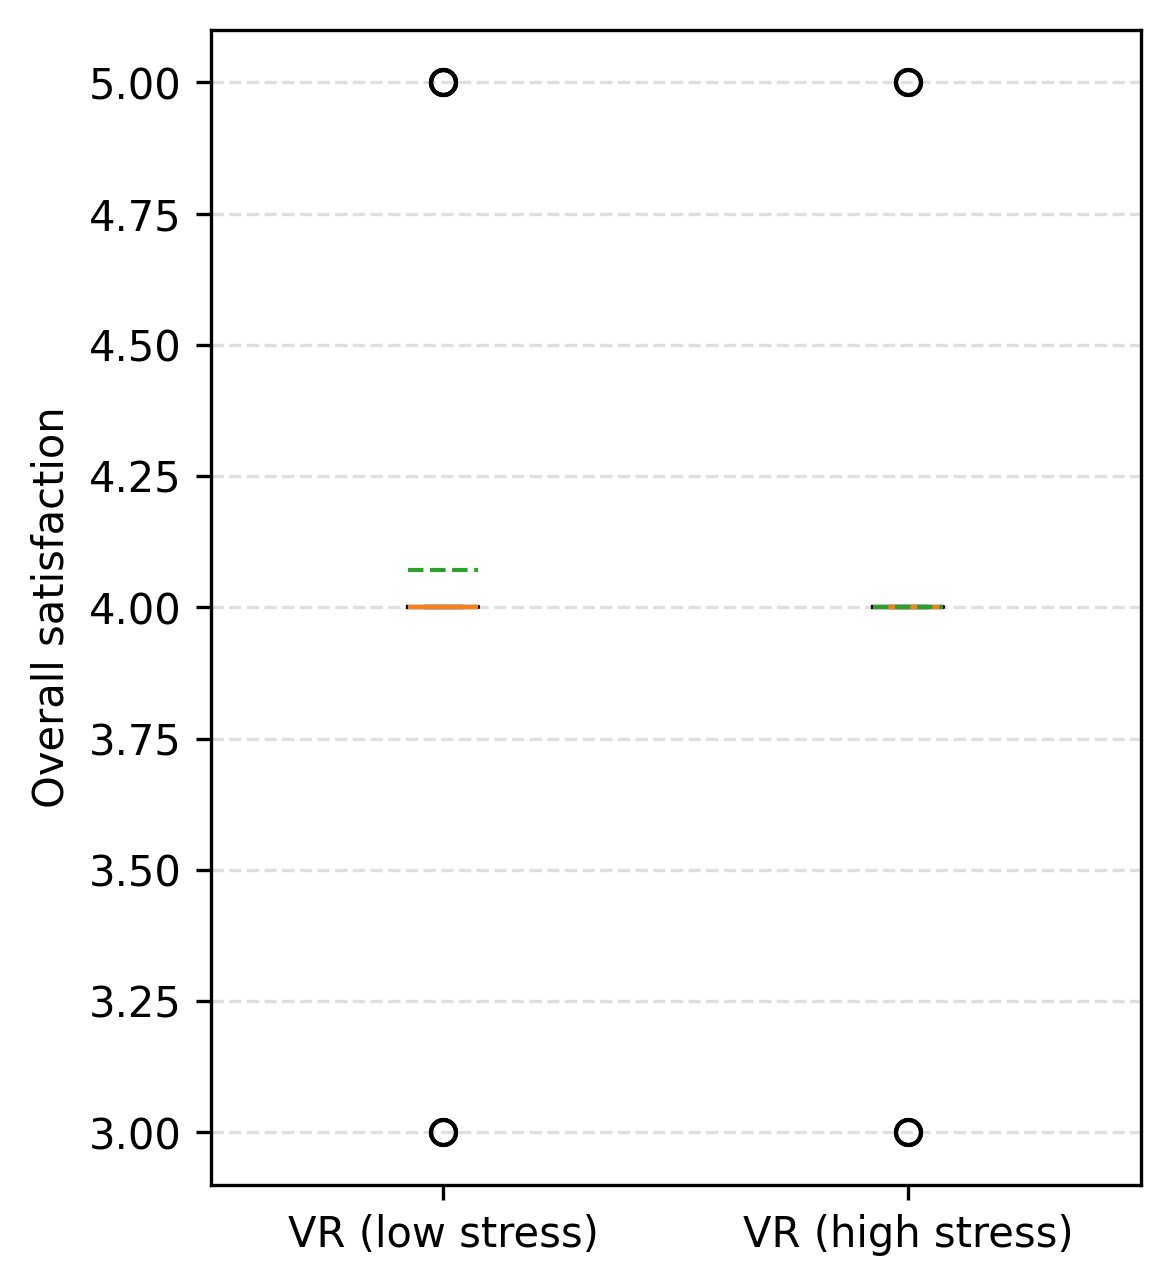
\includegraphics[width=.55\textwidth]{pics/fig8_satisfaction_vr_low_vs_vr_high.png}
  \caption[Overall satisfaction in VR low- vs.\ high-stress subgroups]%
  {Overall satisfaction with VR meditation in low- and high-stress
   subgroups.}
  \label{fig:satisfaction_vr_subgroups}
\end{figure}

\begin{figure}[t]
  \centering
  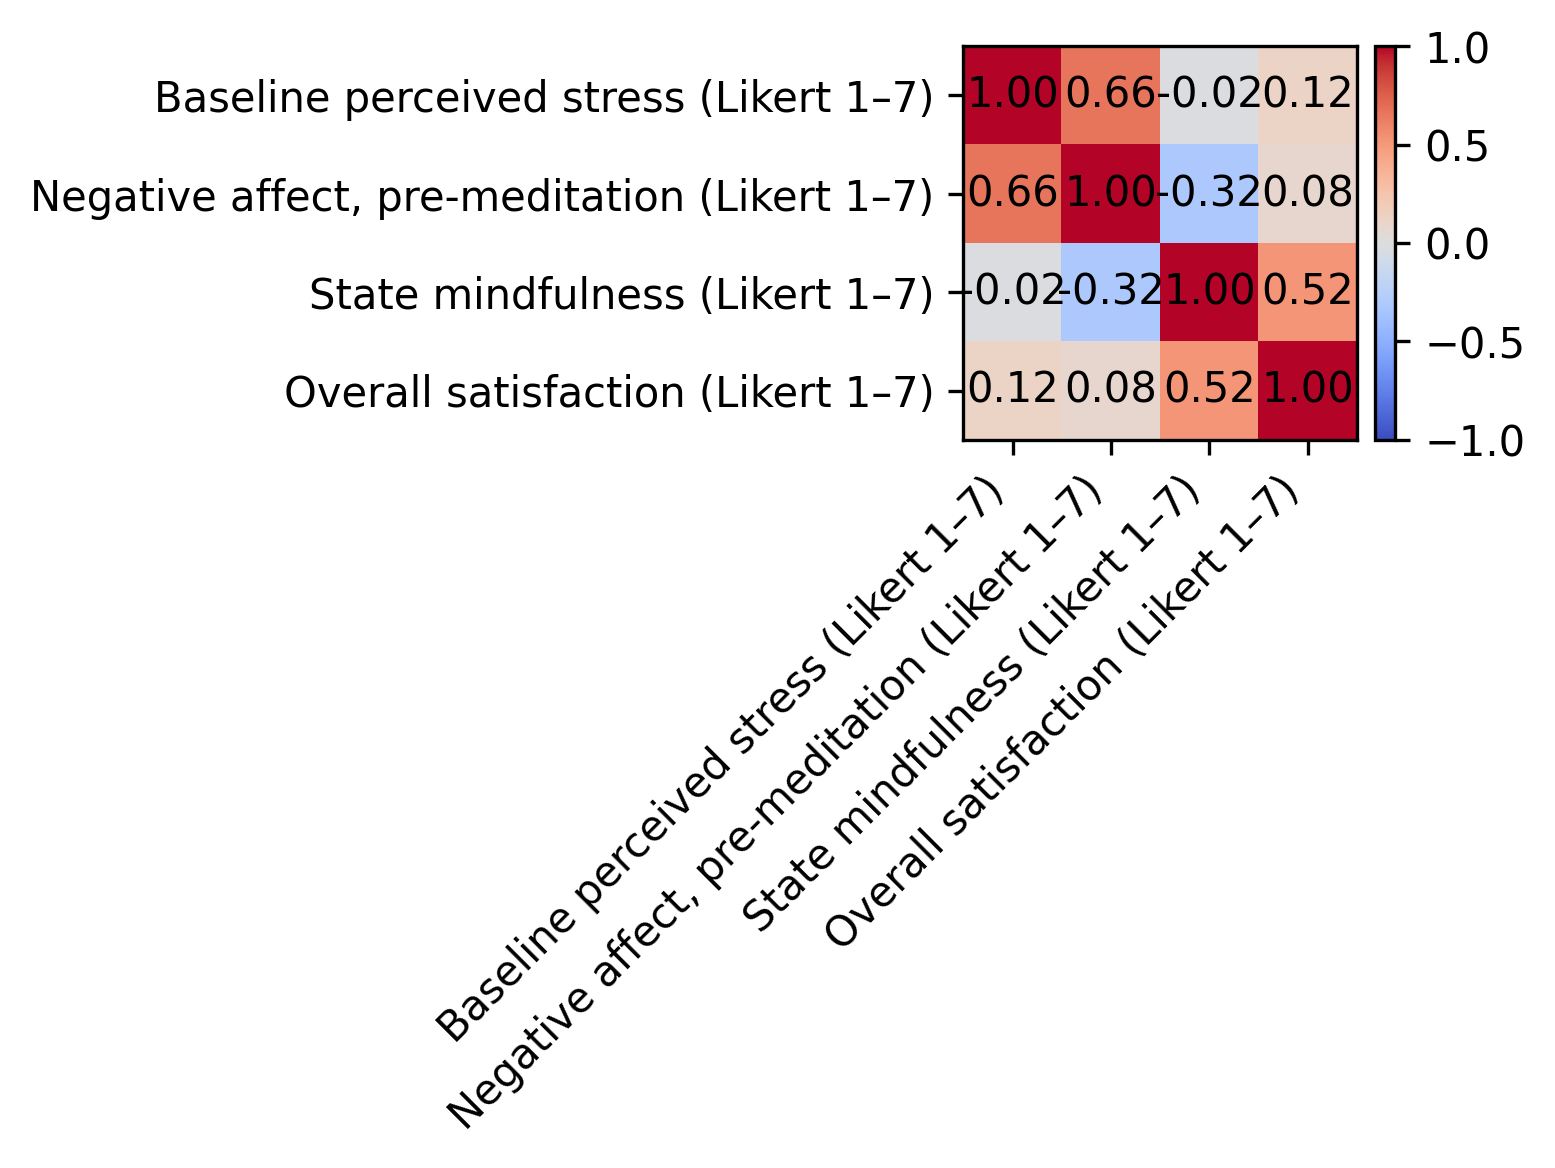
\includegraphics[width=.7\textwidth]{pics/fig9_correlation_questionnaire_scales.png}
  \caption[Correlation matrix of questionnaire scales]%
  {Correlation matrix for the main questionnaire scales (baseline
   perceived stress, negative affect before meditation, state
   mindfulness, and overall satisfaction).}
  \label{fig:questionnaire_correlations}
\end{figure}



